% !TEX root = sob_paper.tex
%% sob_paper.tex --- Star of Bethlehem impossibility proof
%%
%% COMPILATION: use pdflatex (requires texlive-lang-greek / cbfonts for LGR).
%%
%%   IMPORTANT: compile sob_si.tex FIRST so sob_si.aux exists for xr cross-refs.
%%
%%   Local:
%%     pdflatex sob_si.tex && bibtex sob_si && pdflatex sob_si.tex && pdflatex sob_si.tex
%%     pdflatex sob_paper.tex && bibtex sob_paper && pdflatex sob_paper.tex && pdflatex sob_paper.tex
%%
%%   Or with latexmk:
%%     latexmk -pdf sob_si.tex
%%     latexmk -pdf sob_paper.tex
%%
%%   Overleaf: compiler is pdflatex by default --- no change needed.
%%
%% MISSING PACKAGE (local TeX Live basic):
%%   If you get "cuted.sty not found", run once:
%%     sudo tlmgr install sttools
%%
%% GREEK FONT: set \greekfont below to any font installed on your system
%%   that contains the Unicode Greek Extended block (U+1F00--U+1FFF).
%%   macOS:   "Times New Roman" works (ships with Office/macOS)
%%   Linux:   "DejaVu Serif"
%%   Overleaf: "GFS Artemisia"  (default below --- always available on Overleaf)
%%   To install GFS Artemisia locally: tlmgr install greek-fontenc cbfonts gfsartemisia
% !TEX root = sob_paper.tex

\documentclass[sn-nature]{sn-jnl}

%%%% -- Packages ----------------------------------------------------------- (
\usepackage{graphicx}
\usepackage{amsmath,amssymb}
\usepackage{booktabs}
\usepackage{multirow}
\usepackage{xcolor}
%% Engine detection )  must come before inputenc/fontenc/fontspec
\usepackage{iftex}
\usepackage{tabularx}

%% Cross-document references to sob_si.tex (e.g. \ref{subsec:mc_refined}).
%% Compile sob_si.tex first so sob_si.aux exists, then compile sob_paper.tex.
%% TeXLive 2021+ xr handles hyperref's extended \newlabel format correctly.
\usepackage{xr}
\externaldocument{sob_si}

%% -- Greek font selection ---------------------------------------------------
%% Engine-conditional: XeLaTeX uses fontspec (local); pdflatex uses LGR (journal).
\ifPDFTeX
  %% pdflatex path (journal submission system --- TeX Live 2025 full)
  %% Standard utf8 inputenc (LaTeX kernel 2018+) + LGR fontenc for Greek.
  %% Requires greek-fontenc (lgrenc.def, lgrenc.dfu) from texlive-lang-greek.
  \usepackage[utf8]{inputenc}
  \usepackage[LGR,T1]{fontenc}
  \newcommand{\grk}[1]{{\fontencoding{LGR}\selectfont #1}}
\else
  %% XeLaTeX/LuaLaTeX path (local compilation)
  \usepackage{fontspec}
  \newfontfamily\greekfont{Times New Roman}[Script=Greek]
  \newcommand{\grk}[1]{{\greekfont #1}}
\fi
%% Transliteration in italics
\newcommand{\tr}[1]{\textit{#1}}

%%%% -- Document --------------------------------------------------------------
\begin{document}

%% -- Title ------------------------------------------------------------------
\title[The Star of Bethlehem as Legendary Narrative]{%
  Orbital mechanics and corpus linguistics rule out the Star of Bethlehem}

%% -- Author -----------------------------------------------------------------
\author*[1]{\fnm{Aaron} M. \sur{Adair}}\email{adairaar@gmail.com}

\affil*[1]{%
  \orgdiv{Department of Physics},
  \orgname{Massachusetts Institute of Technology},
  \orgaddress{%
    \street{77 Massachusetts Avenue},
    \city{Cambridge},
    \postcode{02139},
    \state{MA},
    \country{USA}}}

%% -- Abstract ----------------------------------------------------------------
\abstract{%
The Star of Bethlehem (Matthew~2:9) depicts a celestial body guiding
travelers southward for two hours, then halting above a specific house.
The feasible set of orbital solutions is shown to be empty.
A heliocentric survey of 529~million configurations spanning all orbit types
and inclinations at every proposed epoch (12--1~BCE) yields zero solutions
satisfying sustained guidance motion, punctual stopping, and the required
azimuth corridor simultaneously.
Monte~Carlo refinement and geocentric surveys confirm the null result.
The impossibility is kinematic: no Keplerian body can sustain southward
apparent motion and subsequently appear stationary above a fixed point.
Independently, all four of Matthew's motion terms
(\grk{προάγω}, \grk{ἵστημι}, \grk{ἐπάνω}, \grk{ἔρχομαι}) are absent
from 24~Greek astronomical texts
(${\approx}\,619{,}000$~words; Fisher combined $p\approx4.5\times10^{-5}$),
while all four characterize guiding-star legendary narratives
(Bayes factor ${\geq}\,10^7$).
Two independent lines of evidence converge: Matthew~2:9 records a legendary
narrative, not an astronomical event.}

\keywords{Star of Bethlehem, orbital mechanics, corpus linguistics, Matthew
2:9, archaeoastronomy, ancient Greek astronomy}

\maketitle

%%%% =======================================================================
\section{Introduction}\label{sec:intro}
%%%% =======================================================================

Testing whether a historical narrative records a real celestial event is
ordinarily a search problem: which known sky object best fits the account?
Here it is shown that such questions can instead be resolved by \emph{demonstration}:
by exhaustively surveying orbital parameter space and demonstrating that the
feasible set is empty.
I apply this paradigm to the most studied ancient astronomical claim
in the Western record and show that two independent lines of evidence, orbital
mechanics and corpus linguistics, converge on the same verdict.

The Star of Bethlehem debate was placed on a renewed scientific footing when Hughes
proposed in these pages that the triple Jupiter--Saturn conjunction of 7~BCE
was the most probable candidate\cite{hughes1976,hughes1979}, a paper that has
accumulated more than 400 citations and sustained the scientific conversation
for five decades. Other proposals include Halley's Comet\cite{kokkinos1989},
a nova\cite{kidger1999,clark1977}, the retrograde motion of Jupiter in
Aries\cite{molnar1999}, and a 5~BCE comet whose possible orbital elements have most
recently been reconstructed from East Asian records\cite{humphreys1992star,matney2025jbaa}.
The present survey explicitly encompasses Matney's proposed orbital parameters
(Monte Carlo Sweep~2; see Methods), confirming that this specific candidate
also falls to the impossibility result.
Systematic reviews show no single candidate satisfies all criteria
simultaneously\cite{adair2013star,schaefer2015}, and the majority position in New Testament
criticism holds that Matthew's infancy narrative is legendary rather than
historical\cite{brown1993,sugihyono2025,merz2015}, though active discussion remains within biblical studies (cf.\ \cite{barthel2015,schaefer2015molnar,freitag1979}).
What has been lacking is not a better candidate but a general demonstration that no orbital solution 
of any class can satisfy the text's kinematic requirements, and a quantitative test of whether 
Matthew's vocabulary belongs to the astronomical register at all.

The critical constraints come from Matthew~2:9:
\grk{ὁ ἀστὴρ οὗ εἶδον ἐν τῇ ἀνατολῇ προῆγεν αὐτούς, ἕως ἐλθὼν
ἐστάθη ἐπάνω οὗ ἦν τὸ παιδίον}
(``the Star which they had seen at its rising was going before them, until,
having arrived, it stood over where the child was'').
The verb \grk{προῆγεν} (imperfect active of \grk{προάγω}) denotes sustained
forward motion ahead of the travelers throughout their journey.
The form \grk{ἐστάθη} (aorist passive of \grk{ἵστημι}), bounded by the
temporal particle \grk{ἕως} (``until''), denotes a completed, punctual
coming-to-rest, a change of state, not a prior condition\cite{adair2013star}. 
The phrase \grk{ἐπάνω οὗ} (``over where'') further
specifies that the stopping occurred directly above a particular
dwelling\cite{adair2013star,heilen2015,bdag2000}.
The two verbs define two physically distinct phases of apparent motion:
a \emph{guidance phase} in which the Star moves ahead of travelers walking
from Jerusalem to Bethlehem, and a \emph{stopping phase} in which it becomes
motionless above a specific house.

Three converging lines of evidence are presented in the order that builds
the argument most naturally.
First, Matthew's own usage of the four motion words across his other 118
Gospel occurrences, zero in any astronomical sense, yields an internal
Bayes factor of ${\approx}\,88{,}000$ against the astronomical reading.
Second, orbital mechanics closes the loose-language escape: the impossibility
is fundamentally geometric: objects in the road corridor appear quasi-stationary
(satisfying the stopping criterion but not guidance), while objects with
sufficient southward motion lie outside it; no Keplerian body can satisfy both
simultaneously.
Third, external corpus-linguistic analysis of 24 Greek astronomical texts
(${\approx}\,619{,}000$ words) places Matthew's vocabulary in the legendary
guiding-star tradition. The linguistic datasets are disjoint, and their
joint Bayes factor remains decisive across the full range of dependence
assumptions tested, from ${\approx}\,6\times10^{3}$ under the most
conservative to ${\approx}\,2.6\times10^{11}$ under strict independence.

%%%% =======================================================================
\section{Methods}\label{sec:methods}
%%%% =======================================================================

\subsection{Reference epoch, site, and coordinate system}

All calculations used the International Celestial Reference System (ICRS,
J2000.0) as the inertial frame. The reference observation window is Julian
Day 1\,719\,755.9 (TDB), corresponding to $\approx\!08{:}00$ local solar
time at Bethlehem ($31.70^\circ$\,N, $35.20^\circ$\,E, 765\,m) on a date
in 5~BCE. The UT1--UTC offset ($\Delta T = 10{,}572$\,s) was derived from
the long-term IERS extrapolation of Morrison \& Stephenson\cite{morrison2004}.
Jerusalem Old City center ($31^\circ 46'$\,N, $35^\circ 14'$\,E) to the
Church of the Nativity, Bethlehem ($31^\circ 42'$\,N, $35^\circ 12'$\,E)
gives a straight-line road bearing of $203^\circ$; the ridge road sweeps
the corridor $[190^\circ, 210^\circ]$ throughout the journey.

Transformation from ICRS to local horizontal (azimuth--altitude) coordinates
used pre-computed East--North--Up (ENU) rotation matrices constructed via
\texttt{astropy}\cite{astropy2022} \texttt{AltAz}$\to$\texttt{SkyCoord.icrs},
incorporating Earth's precession, nutation, and Greenwich Apparent Sidereal
Time at each time step. Applying J2000.0 hour-angle formulae without
precession correction at 5~BCE produces a $25.7^\circ$ systematic azimuth
error; the ENU approach eliminates this. The matrices were validated by
recovering the azimuth of Matney's proposed 5~BCE comet\cite{matney2025jbaa}
($193.7^\circ$) to within $0.01^\circ$ at the reference epoch.

\subsection{Orbit propagation}

Heliocentric positions were computed from osculating orbital elements for
each orbit type. For parabolic orbits ($e=1$), Barker's equation gives the
true anomaly directly. For elliptic ($0\le e<1$) and hyperbolic ($e>1$)
orbits, the mean anomaly $M = n(t-T)$ (or its hyperbolic analogue) was
iterated to Newton--Raphson convergence at tolerance $10^{-12}$\,rad, then
converted to true anomaly. Earth positions came from the JPL DE430
ephemeris\cite{folkner2014}. Geocentric configurations used the same solver
with $GM_\oplus = 3.986\times10^5$\,km$^3$\,s$^{-2}$, with the observer's
GCRS position from \texttt{astropy} at each time step. Heliocentric
positions were vectorised over $\Omega$ and $\omega$ using pre-computed
perifocal unit vectors with \texttt{NumPy}\cite{harris2020}
\texttt{einsum}, enabling evaluation of $72\times72=5{,}184$ orientations
per loop iteration at $5^\circ$ grid resolution.

\subsection{Guidance and stopping criteria}

Three criteria operationalise Matthew's text. (1)~\textit{Visibility:}
object altitude $>5^\circ$ throughout the guidance window
(08:00--10:00 local time, nine 15-min steps). (2)~\textit{Azimuth:}
object azimuth remains within $[190^\circ, 210^\circ]\pm5^\circ$ at every
step, the road corridor from Jerusalem to Bethlehem. (3)~\textit{Motion:}
guidance phase (\grk{προῆγεν}, ongoing) requires minimum apparent angular
velocity $>\omega_\text{thresh}=2^\circ\,\mathrm{h}^{-1}$; stopping phase
(\grk{ἐστάθη}, completed) requires maximum apparent angular velocity
$<\omega_\text{thresh}$ during 10:15--12:00 (eight steps).

The threshold $\omega_\text{thresh}=2^\circ\,\mathrm{h}^{-1}$ is four
times the lunar rate (${\approx}0.5^\circ\,\mathrm{h}^{-1}$ against background
stars) and is detectable by naked eye within minutes; it is deliberately
generous, as any stricter value only strengthens the impossibility result.
Sensitivity analysis across two orders of magnitude ($0.25$--$10^\circ\,\mathrm{h}^{-1}$)
confirms zero configurations satisfy all three criteria at any tested threshold
(Supplementary Table~S1). The lower limit ($0.25^\circ\,\mathrm{h}^{-1}$)
corresponds to motion of ${\approx}5'$ over 20~min, at the practical limit of
unaided naked-eye resolution, ensuring the analysis spans every physically
detectable level of motion.
The upper end of the sweep is independently bounded by a reductio ad absurdum:
the Moon moves at ${\approx}0.5^\circ\,\mathrm{h}^{-1}$ against the background
stars, yet no ancient source describes the Moon as standing still.
Any stopping threshold set \emph{above} the lunar rate would therefore classify
the Moon itself as stationary, plainly inadmissible.
The sensitivity sweep thus brackets the physically meaningful range at both ends:
below by the limit of naked-eye resolution, above by the lunar-rate argument.
The binding constraint is the azimuth
criterion: no Keplerian orbit keeps the object within the road corridor
throughout the 2-hour guidance window; the motion criterion provides
additional independent exclusion at lower thresholds.
Because $\Omega$ and $\omega$ each span all $360^\circ$, the orbital parameter
sweep covers all possible sky positions for a body on the reference date,
making the null result independent of the specific time of night at which the
guidance phase is observed.

\subsection{Survey design and Monte Carlo refinement}

The exhaustive heliocentric survey spanned perihelion distance $q\in[0.02,
1.00]$\,AU (18 values), eccentricity $e$ from 0 to 5 (15 values covering
elliptic, parabolic, and hyperbolic orbits), inclination $i$ from $0^\circ$
to $180^\circ$ in $5^\circ$ steps plus additional fine values near $0^\circ$
to $4^\circ$ (42 total), perihelion epoch offset $\Delta T\in[-60,+60]$\,days
(9 values), and $\Omega$, $\omega$ swept at $5^\circ$ resolution (72 values
each). The outer parameter combinations ($18\times15\times42\times9 =
102{,}060$) multiplied by $72\times72=5{,}184$ orientations yield
$529{,}079{,}040$ total configurations, of which $202{,}372{,}076$ heliocentric configurations were
visible at the reference epoch. Zero satisfied all three criteria
simultaneously (Extended Data Table~1). A separate geocentric survey
spanning LEO to beyond lunar distance ($51{,}200$ configurations;
$28{,}800$ with perigee altitude $>100$\,km) likewise returned zero
solutions.

The $5^\circ$ grid spacing leaves gaps of up to ${\approx}3.5^\circ$
between neighboring points. To confirm the null result is not a grid
artefact, 2.25~million configurations were sampled uniformly in continuous
parameter space in two Monte Carlo sweeps: around the best-fit grid orbit
(Sweep~1: $e\in[0.7,2.5]$, $q\in[0.005,0.15]$\,AU, $i\in[0^\circ,40^\circ]$,
1.5~million configurations) and around Matney's proposed 5~BCE comet
parameters (Sweep~2: 750{,}000 configurations bracketing $q$, $e$, $i$,
$\Omega$, $\omega$ with generous margins). Of 895{,}822 visible
configurations across both sweeps, zero satisfied all three criteria.
The best guidance-phase angular velocity among azimuth-corridor-passing
configurations was $0.006^\circ\,\mathrm{h}^{-1}$, a factor of 330 below
the $2^\circ\,\mathrm{h}^{-1}$ threshold, confirming that the
azimuth--motion trade-off is structural, not an artefact of resolution.

The analysis was repeated at all historically proposed Star of Bethlehem
dates (Halley's Comet, 12~BCE; Jupiter--Saturn conjunction, 7~BCE;
the 5~BCE reference epoch and surrounding months; 1~BCE nova hypothesis),
recomputing Earth positions and ENU matrices from DE430 at each epoch.
Across 79{,}788 visible configurations at seven epochs, zero satisfied all
three criteria (Supplementary Information, \S~S1).

\subsection{Corpus construction and feature classification}
\label{subsec:corpus_methods}

The comparative corpus of 24 ancient Greek astronomical and astrological
texts ($\approx\!619{,}000$ words, 4th~century~BCE through 4th~century~CE)
was assembled from the Thesaurus Linguae Graecae (TLG) electronic
database\cite{tlg}. Three genre classes were distinguished.
\textit{Mathematical astronomy} (Ptolemy \textit{Almagest} and
\textit{Planetary Hypotheses}; Hipparchus; Geminus; Autolycus; Theodosius;
Aristarchus; Cleomedes; Hypsicles) covers geometric and predictive description
of celestial motions. \textit{Astrological application} (Ptolemy
\textit{Tetrabiblos}; Vettius Valens; Hephaestion; Dorotheus;
Pseudo-Manetho; Paul of Alexandria) covers celestial-to-human-destiny
inference; this class is especially important because it is the genre most
likely to employ relational vocabulary of stars guiding or influencing
persons: its null result for all four features closes that alternative
explanation. \textit{Didactic and popularizing works} (Aratus; Eratosthenes;
Achilles Tatius; Theon of Smyrna; Aristotle \textit{Meteorologica};
Theophrastus) complete the coverage. Full corpus inventory is given in
Supplementary Table~S7.

Four lexical features were identified directly from Matthew~2:9, one for each
word Matthew uses to describe the Star's motion, and tested against the corpus.
Feature~A (\grk{προάγω}): the Star ``goes before'' the Magi. The corpus
contains 11 occurrences; all describe positional or temporal
antecedence between celestial bodies (one planet \textit{preceding} another
in longitude) and none describe a celestial body actively guiding human
travelers toward a destination. Feature~B (\grk{ἵστημι}): the Star
``stands''. The corpus contains 121 occurrences across sixteen authors. The
verb is the ordinary vocabulary of the planetary station (\grk{στηριγμός}, the
moment of zero longitudinal velocity in the geocentric model), and Geminus,
Theon of Smyrna and Paul of Alexandria all use it in that sense. What no
occurrence supplies is the complement: in every case what a body stands in, on
or above is a zodiacal sign, a degree, an aspect, a chart angle or a fixed
star, never a terrestrial location. Feature~C (\grk{ἐπάνω}): the Star stands
``over'' a specific dwelling. The corpus contains 40 occurrences, every one of
them zodiacal or geometric; none locates a celestial body above a specific
terrestrial point, for which the invariant astronomical choice is
\grk{ὑπὲρ} (``above'' a zodiacal band or horizon).
Feature~D (\grk{ἔρχομαι}): the Star ``arrives''. The corpus contains 356
occurrences with a celestial subject; every destination governed by
\grk{ἐπί}, \grk{εἰς} or \grk{πρός} is another body or a point in the chart,
never a terrestrial geographic point.

Each feature was searched as a set of exact wordforms covering the full
paradigm of the lemma, one form at a time, with diacritic-sensitive matching
and full results paging: 164 forms for \grk{ἵστημι} and 171 for
\grk{ἔρχομαι} across all four suppletive stems, including the aorist stem that
supplies Matthew's own \grk{ἐλθών}.
Each hit was read in full context and classified by two
independent criteria: (1)~syntactic, is the grammatical subject a celestial
body?; (2)~semantic, does the usage match the specific sense in Matthew~2:9?
All classification decisions are recorded passage-by-passage in
Supplementary Table~S8, enabling independent verification by any reader
with TLG access.

\subsection{Statistical framework and Bayes factors}
\label{subsec:stats_methods}

Fisher's exact test (one-sided) was applied to each $2\times2$ contingency
table of corpus-hit classifications. The Laplace-smoothed probability under
$H_\text{astro}$ for each feature is $p_i = 1/(n_i+1)$, where $n_i$ is the
number of corpus hits and the numerator 1 reflects zero positive matches.
The joint Fisher combined statistic $X=-2\sum_i\ln p_i = 33.76$ on
$\mathrm{df}=8$ gives $p_\text{Fisher}\approx4.5\times10^{-5}$. Feature
independence was checked by Gaussian copula simulation ($2\times10^6$~Monte
Carlo draws) and Brown's variance-corrected method across equicorrelation
values $\rho=0$--$0.95$; the joint $p$ remains below 0.05 across the whole tested range, to $\rho=0.95$ (Supplementary Table~S10).

The guiding-star comparison corpus comprises four independently attested
pre-Matthean or contemporaneous traditions: Virgil \textit{Aeneid}
2.687--711; the Timoleon flame tradition (Plutarch \textit{Tim.}~8 and
Diodorus Siculus 16.66.3, counted as one tradition from a common source);
Lucian \textit{Navigium}~7,~9; and the Israelite pillar-of-fire tradition
(Exodus 13:21--22; Numbers 9:15--23). The \textit{Protoevangelium of James}~21 is excluded as a
derivative of Matthew~2:9. An omen corpus (Josephus \textit{Jewish
War}~6.289; Dio Cassius 54.29.8; PGM~I.54--95) is included in sensitivity
analyses. Each tradition was scored on features A--D by narrative function;
scores are given in Supplementary Table~S11. The corpus Bayes factor is:
\begin{equation}
  \mathrm{BF}_\text{corpus}
    = \prod_{i\in\{A,B,C,D\}}
      \frac{P(\text{feature}_i \mid H_\text{guide})}
           {P(\text{feature}_i \mid H_\text{astro})},
\end{equation}
where each probability uses Laplace smoothing over the respective corpus
($N=4$ guiding-star traditions; $N=24$ astronomical texts), giving
$\mathrm{BF}_\text{corpus}\approx3.0\times10^{6}$ under strict independence,
falling to ${\approx}\,6\times10^{1}$ once both dependence corrections are
applied at their strongest (Supplementary Table~\ref{tab:bfsens}).

An independent within-Matthew Bayes factor was derived from Matthew's own
Gospel. Every occurrence of the four features outside Matthew~2:9 was
identified from the BibleHub interlinear (Strong's numbers G4254, G2476,
G1883, G2064), cross-checked against NA28/SBLGNT lemmatization.
Across $n=5+20+7+86=118$ other Matthean occurrences, zero use any of the
four words in an astronomical sense. The Laplace-smoothed likelihood ratio
for feature $i$ under $H_\text{guide}$ versus $H_\text{astro}$ is
$\mathrm{BF}_i=n_i+1$, giving
$\mathrm{BF}_\text{Matthew}=6\times21\times8\times87=87{,}696$.
Because this analysis draws entirely from Matthew's Gospel while
$\mathrm{BF}_\text{corpus}$ draws from the TLG and guiding-star traditions,
the datasets are disjoint and the factors are treated as conditionally
independent, as they derive from non-overlapping corpora and distinct
sampling frames.
Their product is the joint Bayesian update from the linguistic evidence
considered here. Because both factors are products over the same four
features, and those features are four properties of a single clause, the
result is reported as a sensitivity range rather than a point estimate:
$\mathrm{BF}_\text{joint}$ spans $6.4\times10^{3}$ to $2.6\times10^{11}$
across the dependence assumptions tabulated in Supplementary
Table~\ref{tab:bfsens}, with a central range of $2.5\times10^{5}$ to
$6.0\times10^{7}$. Every value tested exceeds the Jeffreys threshold for
decisive evidence by at least an order of magnitude.
Features A--D co-occur in the same verse and are treated as conditionally
independent in both BF calculations. Under positive correlation (plausible,
since all four features reflect the same register choice), features absent
together in the corpus tend to remain absent together, so
$P(\text{data}\mid H_\text{astro})$ increases relative to the product of
marginals, raising the BF denominator and thereby \emph{reducing}
$\mathrm{BF}_\text{corpus}$. The independence assumption therefore gives an
upper bound on $\mathrm{BF}_\text{corpus}$; the Gaussian copula simulation
confirms the evidence remains substantial up to inter-feature correlation
$\rho=0.95$.

\subsection{Software and reproducibility}

All orbital-mechanics and statistical analyses were performed in Python~3.12
using \texttt{astropy}\cite{astropy2022} (coordinate transformations,
ephemeris access, time systems), \texttt{NumPy}\cite{harris2020} (vectorised
array operations), \texttt{SciPy}\cite{virtanen2020} (Fisher's exact test,
Newton--Raphson utilities), and \texttt{matplotlib}\cite{hunter2007}
(figures). Code and data needed to reproduce all figures and tables are
available at \url{https://github.com/adairaar/sob_astro_test}. Key scripts include:
\texttt{sob\_proof\_fine.py} (529-million-configuration heliocentric survey);
\texttt{sob\_mc\_refined.py} (Monte Carlo refinement);
\texttt{sob\_epoch\_robustness.py} (multi-epoch analysis);
\texttt{corpus\_pvalue.py} (Fisher combined p-value and Gaussian copula independence robustness test);
\texttt{guiding\_star\_bayes.py} (corpus and within-Matthew Bayes factor computation).
Sky-position results at representative epochs were independently cross-validated
against Stellarium planetarium software\cite{stellarium2021}, which implements
the same Keplerian propagation model; computed positions agreed to within
observational tolerances at all tested epochs.

\subsection{Use of artificial intelligence}

An AI assistant (Claude, Anthropic) was used to write and revise the analysis
code, to suggest statistical treatments including the Kish design-effect
correction and the Gaussian copula sensitivity analysis, and to assist in
drafting and editing text. All code was reviewed and executed by the author,
all reported quantities were checked against independent calculation, and all
interpretive claims and final wording are the author's own. The code is
available as described under Code availability, so that every number reported
here can be reproduced independently.

%%%% =======================================================================
\section{Results}\label{sec:results}
%%%% =======================================================================

\subsection{Matthew's own vocabulary excludes the astronomical reading}
\label{subsec:within_matthew_results}

A necessary condition for the astronomical reading of Matthew~2:9 is that the
four motion words can carry astronomical senses. The author's own usage
elsewhere in his Gospel provides direct evidence against this: across all 118
other occurrences of \grk{προάγω}, \grk{ἵστημι}, \grk{ἐπάνω}, and
\grk{ἔρχομαι} in Matthew, zero appear in any sense compatible with an
astronomical body (Methods; full passage data in Supplementary Information).

\grk{Προάγω} appears five more times (14:22; 21:9$\times$2; 26:32; 28:7),
always transitive with a human direct object, identical syntax to
\grk{προῆγεν αὐτούς} in Matt~2:9; the intransitive positional-antecedence
sense the astronomical reading requires is unattested in Matthew, nor does 
Matthew use other terms for ``leading" that have an astronomical register 
(e.g., the intransitive \grk{προηγέομαι}).
\grk{Ἵστημι} appears 20 more times with persons or objects at named physical
locations; the mathematical stationary point is never its referent anywhere in
the Gospel.
\grk{Ἐπάνω} appears seven more times denoting physical contact or immediate
proximity; at Matt~28:2 an angel sits \grk{ἐπάνω} the rolled-away stone, a
heavenly being in point-contact with a terrestrial object, the same register
as Matt~2:9. \grk{Ὑπέρ} would be the expected Greek preposition for an astronomical body. 
On its own, read literally, \grk{ἐπάνω} disqualifies the astronomical 
reading: a celestial body cannot be ``over'' a specific house in the sense of physical 
contact or immediate proximity. Nonetheless, I will conservatively only consider word 
counts in Matthew's own idiolect, not the semantic content of the words themselves, 
in the Bayes factor calculation below.
\grk{Ἔρχομαι} appears 86 more times with persons or agents
arriving at terrestrial locations; never with a celestial body reaching a
zodiacal position or celestial coordinate. Another verb could be used for ``arriving'' 
in astronomical texts (e.g., \grk{καταντάω}), but Matthew never uses it.

Using Laplace smoothing, the Bayes factor for feature~$i$ from Matthew's own
idiolect is $\mathrm{BF}_i = n_i + 1$ (non-astronomical uses $n_i$, zero
astronomical uses). The joint within-Matthew Bayes factor is:
\begin{equation}
  \mathrm{BF}_\text{Matthew}
    = \prod_i (n_i + 1)
    = 6 \times 21 \times 8 \times 87
    = 87{,}696.
  \label{eq:bf_matthew_main}
\end{equation}
Matthew's own vocabulary disfavors the astronomical reading at $\approx$88{,}000 to~1.

The key epistemic point is what BF\textsubscript{Matthew} measures: not that Matthew never
discusses astronomy elsewhere, he rarely has occasion to, but that when
describing the Star's motion he consistently reaches for words the external
corpus identifies as belonging to the non-astronomical register. This reading
is not a modern analytical artifact: no ancient or medieval commentator
interpreted the Star's motion in Matt~2:9 as a natural astronomical
phenomenon\cite{adair2012}; every pre-modern interpreter understood the Star
as not astronomical or astrological, but miraculous. The
following sections test the remaining escape route: whether colloquial or
imprecise language could nonetheless describe a real celestial event.

\subsection{Geometric and temporal constraints from Matthew 2:9}
\label{subsec:constraints}

The Magi traveled from Jerusalem (Old City center: $31^\circ 46'$\,N,
$35^\circ 14'$\,E) to Bethlehem (Church of the Nativity: $31^\circ 42'$\,N,
$35^\circ 12'$\,E), approximately 8\,km along the ancient ridge road to the
south-southwest. The straight-line bearing is $203^\circ$; because the road
deviates around the central ridge, the actual azimuth of travel sweeps from
approximately $190^\circ$ to $210^\circ$ along the route. I therefore adopt a
road-corridor guidance criterion: the Star's azimuth must remain within
$[190^\circ, 210^\circ] \pm 5^\circ$ throughout the 2-hour journey
(Fig.~\ref{fig:sky}).

The criterion for \grk{προῆγεν} (``was going before'') is not merely
positional: a stationary object at the right azimuth cannot ``go before'' 
(let alone guide) travelers\cite{adair2013star}.
I therefore require the Star to exhibit perceptible southward motion throughout
the guidance phase. I adopt an angular-velocity floor of
$\omega_\mathrm{thresh} = 2^\circ\,\mathrm{h}^{-1}$ (4$\times$ the Moon's
motion relative to background stars, ${\approx}\,0.5^\circ\,\mathrm{h}^{-1}$,
which Babylonian astronomers monitored routinely). This threshold is
deliberately generous: naked-eye resolution is approximately $1'$, so motion
is detectable over a 30-minute observation at any rate above
${\approx}\,0.03^\circ\,\mathrm{h}^{-1}$, thirty-fold below this floor.
Choosing any stricter threshold only strengthens the impossibility conclusion.
The \textit{guidance criterion} is therefore: (i)~azimuth within the road
corridor for the full journey, and (ii)~apparent angular velocity
$> 2^\circ\,\mathrm{h}^{-1}$ throughout.

Walking pace on hilly terrain yields a journey time of approximately 2~hours.
I locate this journey in the pre-dawn hours of a date in 5~BCE (Julian Day
1\,719\,755.9, $\approx\!08{:}00$--$10{:}00$ local solar time), consistent
with the most recently proposed candidate\cite{matney2025jbaa}. Following
arrival at Bethlehem, the Star must appear stationary over the specific house
(\grk{ἐστάθη ἐπάνω}, ``stood over'').
The verb \grk{ἐστάθη} is passive aorist, denoting a punctual \emph{change of state}:
the Star transitioned into standing still, not that it was stationary from the outset.
An object whose angular rate falls below $\omega_\mathrm{thresh}$ throughout the entire
observation window, including during the guidance phase, cannot satisfy this aorist
stopping event, because no transition from motion to rest has occurred.
The stopping criterion therefore carries an implicit sequential requirement:
the angular rate must have been \emph{above} $\omega_\mathrm{thresh}$ during the
guidance phase and must fall \emph{below} it afterward.
Guidance before stopping, in that order, is a formal constraint of the analysis.
The \textit{stopping criterion} is maximum apparent angular velocity below
$2^\circ\,\mathrm{h}^{-1}$ during the $10{:}00$--$12{:}00$ window immediately
following the journey, the same threshold $\omega_\mathrm{thresh}$, applied as
an upper rather than lower bound. A sensitivity sweep across thresholds
$\omega_\mathrm{thresh} \in \{0.25, 0.5, 1, 2, 5, 10\}^\circ\,\mathrm{h}^{-1}$
yields zero satisfying configurations at every value tested (Supplementary
Information, Table~S1).

\begin{figure}[htbp]
  \centering
  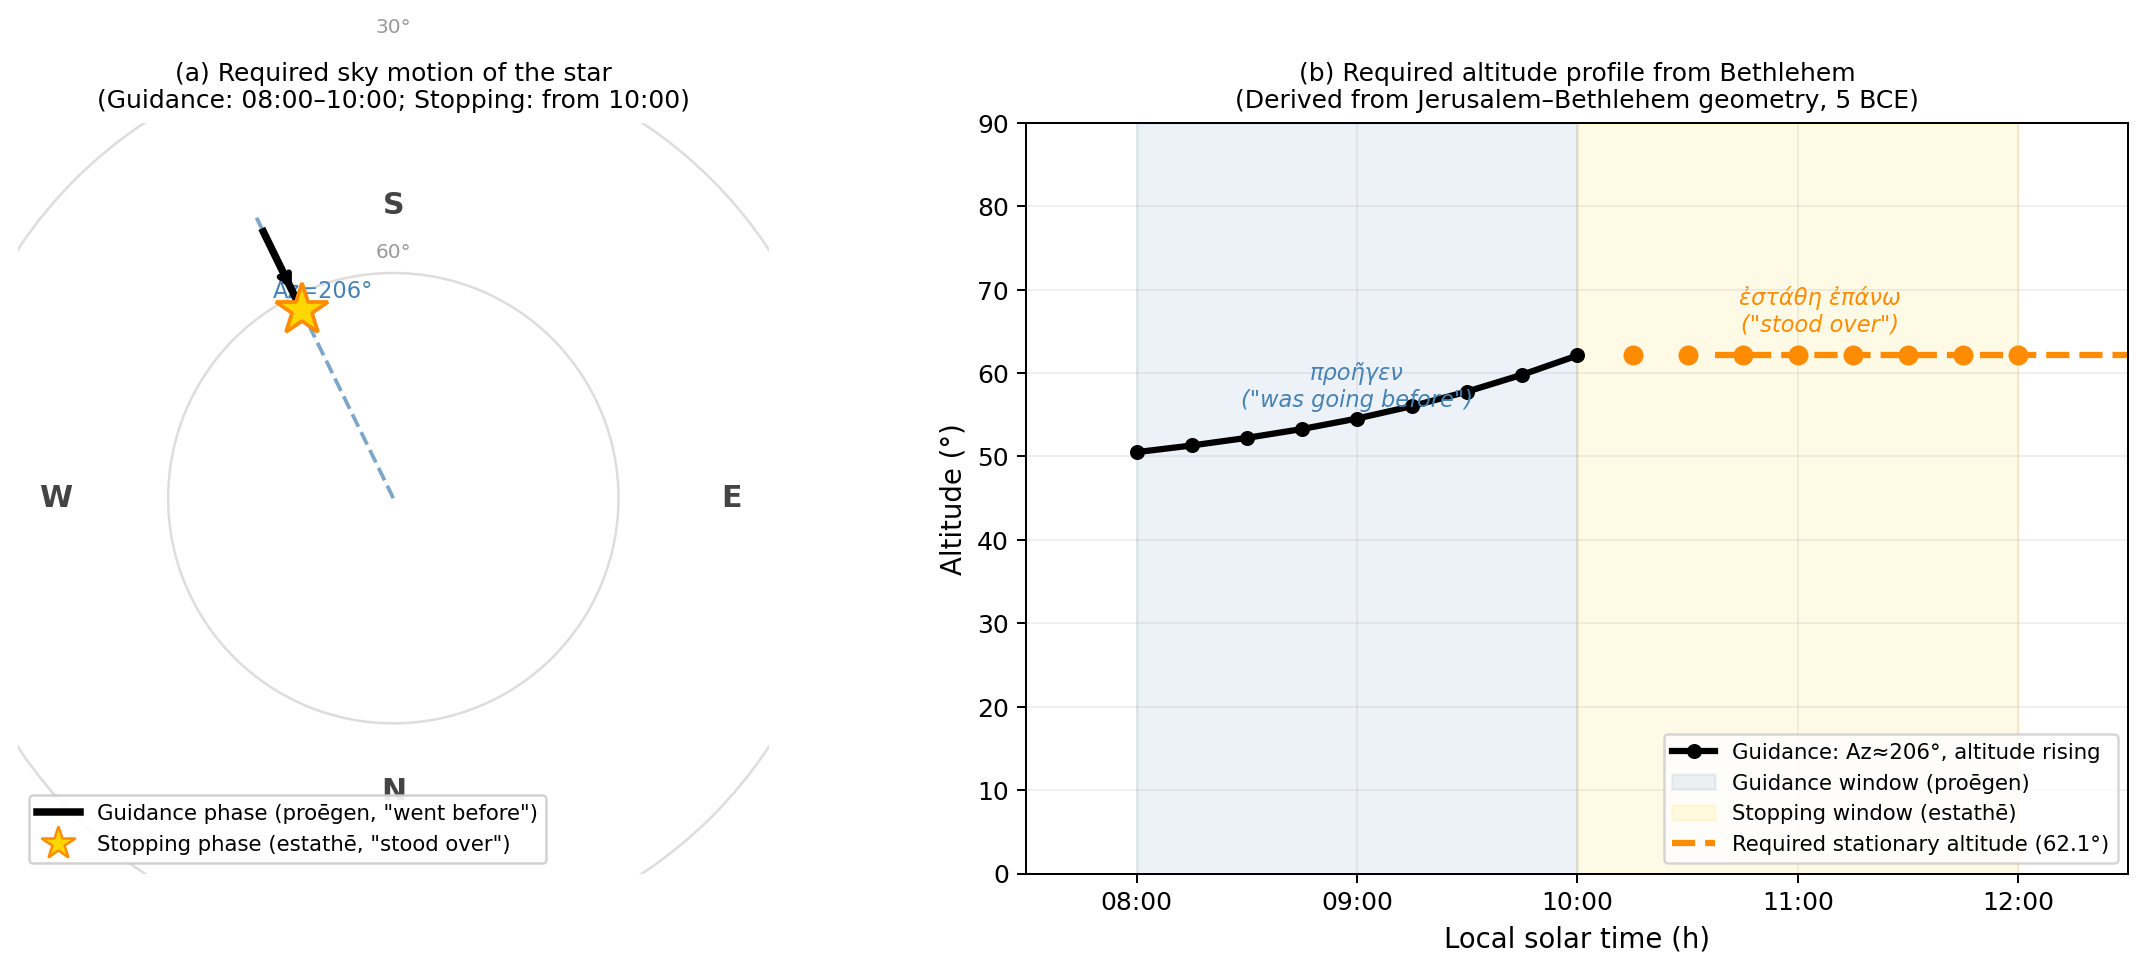
\includegraphics[width=\linewidth]{figure_paper1_sky_geometry}
  \caption{\textbf{Observational constraints from Matthew 2:9.}
    a)~Polar sky chart showing the required apparent motion: during
    the 2-hour guidance phase (\grk{προῆγεν}, ``was going before''), the Star
    must move visibly southward with azimuth within the road corridor
    $[190^\circ, 210^\circ]$ toward Bethlehem; it then appears stationary
    over a specific house (star symbol, \grk{ἐστάθη}, ``stood over'').
    Altitude is not constrained during stopping (any altitude above the horizon
    is acceptable): scholarly interpretations of ``stood over'' range from
    just above the horizon to zenith.
    b)~The road corridor $[190^\circ, 210^\circ]$ in the local sky
    from Bethlehem. The straight-line bearing is $203^\circ$; the road deviates
    around the central ridge, sweeping between $190^\circ$ and $210^\circ$.}
  \label{fig:sky}
\end{figure}

\subsection{Kinematic demonstration of incompatibility}\label{subsec:kinematic}

The argument in this subsection is a mathematical demonstration, not a numerical
result. The conceptual core is geometric: the south-southwest bearing of the
Jerusalem--Bethlehem route means that any Keplerian body within the road
corridor appears quasi-stationary throughout (satisfying the stopping criterion
but not guidance), while any body with sufficient southward apparent motion
lies outside the corridor, a mutual exclusion. The analysis below makes this
precise, establishing from the geometry of the bearing and Earth's rotation
rate alone that the required ICRS angular velocities during guidance and
stopping are unachievable for any heliocentric body, and that the transition
between them is additionally forbidden by gravitational dynamics. The numerical
surveys in the following subsections are corroborative.

Converting the two observational phases into ICRS velocity requirements via
pre-computed East--North--Up (ENU) rotation matrices (Methods), the argument
proceeds as follows.

\textit{Stopping phase ($10{:}15$--$12{:}00$).}~An object motionless in the
local horizontal frame (``stood over'') must, because the local AltAz
frame co-rotates with Earth, sweep through ICRS at the sidereal rate.
At a representative stopping altitude of $45^\circ$ (az\,$=\,200^\circ$,
Bethlehem latitude $31.7^\circ$N), this is $\omega_\mathrm{stop} = 14.76^\circ\,\mathrm{h}^{-1}$
(Table~\ref{tab:kinematics}). Such a criterion already excludes fixed stars, novae, and planets, 
which all move at approximately the sidereal rate.

\textit{Guidance phase ($08{:}00$--$10{:}00$).}~An object visibly ``going before''
travelers at the minimum rate $2^\circ\,\mathrm{h}^{-1}$ in local AltAz
along azimuth $200^\circ$ yields, by vectorial addition of the sidereal rate,
$\omega_\mathrm{guide} = 15.55^\circ\,\mathrm{h}^{-1}$ in ICRS.

\textit{Primary impossibility (literal interpretation).}~Both ICRS values
(${\approx}\,15^\circ\,\mathrm{h}^{-1}$) are unachievable for standard heliocentric bodies.
Since $\omega_\mathrm{ICRS} = V_\perp/d$ with $V_\perp \propto d$, for any
naked-eye heliocentric candidate with $d \gtrsim 0.1$\,AU, the stopping
state requires $V_\perp \gtrsim 1{,}070$\,km\,s$^{-1}$ (e.g.\ ${\approx}\,5{,}560$\,km\,s$^{-1}$
at Mars opposition; ${\approx}\,44{,}900$\,km\,s$^{-1}$ at Jupiter), far above any known
solar-system speed. The very close flyby regime ($d\!\sim\!0.003$\,AU) reduces
the requirement to $V_\perp\!\sim\!30$\,km\,s$^{-1}$ (achievable in principle),
but apparent motion there is overwhelmingly diurnal, indistinguishable from any
fixed star, and Matney's proposed comet occupies a fully sunlit sky throughout
the relevant window.

The close-flyby regime is thus the one case the analytic argument does not
settle. It is therefore surveyed numerically rather than assumed away. Three
surveys bear on it, and they agree.

A nighttime survey of 10~million Monte Carlo orbits yields 66 genuine close
flybys. None satisfies the guidance\,$\to$\,stopping criterion
(Supplementary~\S\,\ref{subsec:closeflyby}). A numerical optimizer over
100~restarts reaches at most $0.58$~h of contiguous guidance, against a
requirement of $1.0$~h. A later campaign of $10^{9}$ orbits yields $6{,}116$
close flybys and tests each against $525$ combinations of the guidance and
stopping parameters; none passes
(Supplementary~\S\,\ref{subsec:sweep}).

Full derivation and distance table in Supplementary~\S\,S1.9.

\textit{Secondary constraint (astronomical-vocabulary interpretation).}~Even
under the more permissive reading that the verbs describe motion relative to
the stellar background, the transition between the two states is forbidden.
The guidance and sidereal-tracking trajectories differ in direction in ICRS,
requiring an impulsive $\Delta v \approx 1.5$\,km\,s$^{-1}$ at $d = 0.0026$\,AU.
Under Earth gravity ($a_\oplus = 2.6\times10^{-6}$\,km\,s$^{-2}$) this
requires ${\approx}\,158$\,h; the deceleration time scales as $r^3$,
making the problem strictly worse at any greater distance.
The corpus-linguistic analysis below independently closes this interpretive
retreat by showing that the verbs belong to the narrative, not astronomical,
register.

\begin{table}[h]
\caption{Kinematic parameters for the guidance and stopping phases at three
representative stopping altitudes (azimuth $200^\circ$, Bethlehem).
$\omega_\mathrm{guide}$: ICRS angular velocity of a star rising at the
minimum detectable rate ($2^\circ\,\mathrm{h}^{-1}$ in local AltAz) along
azimuth $200^\circ$.
$\omega_\mathrm{stop}$: ICRS angular velocity of a star stationary in local
AltAz (sidereal tracking).
$\Delta v$ at $r = 0.0026$\,AU (Matney's closest approach): minimum
transverse velocity change required for the phase transition.}\label{tab:kinematics}
\begin{tabular}{@{}lccccc@{}}
\toprule
Alt.\ ($^\circ$) & $\omega_\mathrm{guide}$ ($^\circ\,\mathrm{h}^{-1}$) &
  $\omega_\mathrm{stop}$ ($^\circ\,\mathrm{h}^{-1}$) &
  $\Delta\omega$ ($^\circ\,\mathrm{h}^{-1}$) &
  $\omega_\mathrm{stop}/\omega_\mathrm{thresh}$ &
  $\Delta v$ (km\,s$^{-1}$) \\
\midrule
20 & 13.44 & 12.34 & 1.10 & 6.2$\times$ & 2.07 \\
45 & 15.55 & 14.76 & 0.79 & 7.4$\times$ & 1.50 \\
60 & 15.68 & 15.02 & 0.66 & 7.5$\times$ & 1.24 \\
\bottomrule
\end{tabular}
\end{table}

\subsection{Exhaustive survey of heliocentric orbits}
\label{subsec:helio}

The null result is driven primarily by the geometric incompatibility between
sustained southward motion and corridor confinement; the stopping criterion
then eliminates the small residual near-matches that pass azimuth screening.
I conducted an exhaustive heliocentric survey with a fine angular grid.
The longitude of ascending node~$\Omega$ and argument of perihelion~$\omega$
were sampled at $5^\circ$ intervals ($72 \times 72 = 5{,}184$ orientations
per outer combination) across eccentricities
$e \in \{0, 0.1, 0.2, 0.3, 0.5, 0.7, 0.8, 0.9, 0.95, 0.99, 1.0, 1.1,
1.5, 2.0, 5.0\}$ (elliptic through hyperbolic, spanning the eccentricity
range of the known interstellar objects
1I/\textquoteleft{}Oumuamua ($e \approx 1.20$)\cite{meech2017} and
2I/Borisov ($e \approx 3.36$)\cite{guzik2020}), perihelion distances
$q \in \{0.02, 0.03, 0.04, 0.05, 0.07, 0.10, 0.15, 0.20, 0.25, 0.30,\allowbreak
0.35, 0.40, 0.50, 0.60, 0.70, 0.80, 0.90, 1.00\}$\,AU (18 values,
reaching Earth's orbital distance), inclinations $0^\circ$ to $180^\circ$
in $5^\circ$ steps with additional fine sampling near $0^\circ$
(42 values total; Supplementary Information~\S\ref{subsec:mc_refined}), and perihelion epoch offsets
$\Delta T \in \{-60, -40, -20, -10, -5, +5, +10, +20, +60\}$~days (9
values), yielding $18 \times 15 \times 42 \times 9 = 102{,}060$ outer
combinations and $102{,}060 \times 5{,}184 = 529{,}079{,}040$ total
configurations sampled. Of $202{,}372{,}076 \pm 0.1\%$ visible configurations
(object above $5^\circ$ altitude throughout the guidance window), zero
simultaneously satisfy all three criteria: road-corridor azimuth,
guidance motion $> 2^\circ\,\mathrm{h}^{-1}$, and stopping motion
$< 2^\circ\,\mathrm{h}^{-1}$ (Table~\ref{tab:survey}).
Census counts of this kind carry a tolerance of order $0.1\%$ because
configurations lying within numerical noise of a threshold may be classed
either way under different ephemeris implementations; the count satisfying
all criteria is exactly zero and is reproduced identically across builds
(Supplementary~\S\,\ref{subsec:reproducibility}).
The best azimuth corridor score is $0.015^\circ$ inside the corridor
(orbit $e=1.1$, $q=0.03$~AU, $i=10^\circ$, identified by the
complementary fine-grid orbit inversion of Section~\ref{subsec:inversion}),
yet that configuration's angular velocity is $0.23^\circ\,\mathrm{h}^{-1}$, an
order of magnitude below the required guidance motion. Configurations that come closest to
the azimuth criterion are found to be nearly stationary: they satisfy the stopping
criterion but have angular velocities far below the
$2^\circ\,\mathrm{h}^{-1}$ guidance-motion threshold, because a
stationary object cannot \grk{προάγειν} (``go before'') anyone.

To verify this null result is not a grid-spacing artefact, I performed two
Monte Carlo refinement sweeps (Supplementary Information~\S\ref{subsec:mc_refined}
and Fig.~S1). Sweep~1 (1.5~million configurations near the best-fit grid orbit)
found zero of 601,150 visible configurations satisfying all criteria; the
closest azimuth match had guidance velocity of $0.006^\circ\,\mathrm{h}^{-1}$, a
factor of ${\sim}330$ below threshold. Sweep~2 (750,000 configurations near
Matney's proposed 5~BCE comet) found zero of 294,672 visible configurations,
with the best-azimuth candidate lying outside the road corridor entirely. No
fine-tuning yields a viable solution: the incompatibility is structural.

\subsection{Survey of Earth-orbiting objects}\label{subsec:geocentric}

For geocentric objects the primary impossibility of Section~\ref{subsec:kinematic}
does not apply: an Earth-orbiting body \emph{can} in principle exhibit
perceptible motion and then appear to slow, because its apparent motion is
governed by its orbital velocity relative to the ground observer rather than
by the sidereal rate. The geocentric case therefore requires a separate analysis
in ground-frame AltAz coordinates.

The Moon, the only known natural geocentric body in antiquity, reaches
$\omega_\mathrm{max} = 0.61^\circ\,\mathrm{h}^{-1}$ at perigee, falling short
of the $2^\circ\,\mathrm{h}^{-1}$ guidance threshold by a factor of three.
A comprehensive survey of 28,800 hypothetical geocentric orbit configurations
(the physically admissible subset (perigee altitude $>100$\,km) of 51,200 total
grid configurations; semi-major axes from 7,000~km to 500,000~km,
eccentricities 0--0.99, all inclinations and orientations;
Supplementary~\S\,S1.10) finds zero
configurations satisfying all criteria with a realistic stopping threshold
$\omega_\mathrm{stop} < 0.20^\circ\,\mathrm{h}^{-1}$.
The only configurations approaching even the loose threshold
($\omega_\mathrm{stop} < 0.50^\circ\,\mathrm{h}^{-1}$) are equatorial orbits
near geosynchronous distance exhibiting the meridian-transit azimuth artifact:
as any equatorial object crosses the meridian, its azimuth rate passes through
zero briefly while altitude continues to change, the same geometric effect
described for Matney's comet, not a physical deceleration.
All 28,800 physically admissible geocentric configurations have the object
above $5^\circ$ altitude during at least one evaluated interval, so all
contribute to the visible count.
Combined with the heliocentric survey, 202,400,876 visible configurations
spanning all orbit types yield zero solutions (Extended Data Table~1;
Figs.~\ref{fig:azmotion} and~\ref{fig:scatter}).

It is worth being explicit about which requirement carries the result, because
the criteria are not equally demanding when taken singly.  Considered on its
own, stopping is easy: in the fine survey $201{,}505{,}224$ of the
$202{,}372{,}076$ visible configurations, better than $99.5\%$, are moving
slowly enough at some moment to qualify.  Nor is the difficulty simply that
each criterion is individually rare.  What no orbit achieves is the
\emph{conjunction}: guidance along the road corridor followed by a stop.
Not one configuration in $5.29\times10^{8}$ manages both, and the failure is
not marginal: the azimuth requirement alone admits zero configurations at
every stopping threshold tested across two orders of magnitude
(Supplementary Table~S1), and the best candidate located by direct
optimization falls short of the required guidance interval by $0.04$\,h.

This matters for how the result should be read.  A sceptical reader may prefer
a looser construal of \grk{ἐστάθη} (taking the Star merely to have lingered,
rather than to have halted in the strict sense) and on such a reading the
stopping criterion alone would be weak.  The conjunction is untouched by that
move.  Whatever latitude is granted to ``stood still,'' the object must first
have guided travelers southward along a fixed bearing and then have ceased
doing so, and it is the ordered pair of behaviors, not either member of it,
that Keplerian motion cannot supply.

Figure~\ref{fig:azmotion} demonstrates the two-criterion near-impossibility:
satisfying the road-corridor direction \emph{and} the guidance-motion requirement
simultaneously is already unachievable. Figure~\ref{fig:scatter} shows that
adding the stopping criterion completes the impossibility. The characteristic
slope-1 diagonal in that figure is a rigorous consequence of Kepler's second
law: apparent angular velocity $\omega_\mathrm{app} = V_\perp/d$ changes by at
most $\lesssim\!4\%$ over any four-hour window for bodies with
$d \gtrsim 0.5$\,AU (Supplementary~\S\,S1.8), so the sole mechanism that could
break this conservation, a retrograde stationary point, is geometrically
excluded by the azimuth constraint.

\begin{figure}[htbp]
  \centering
  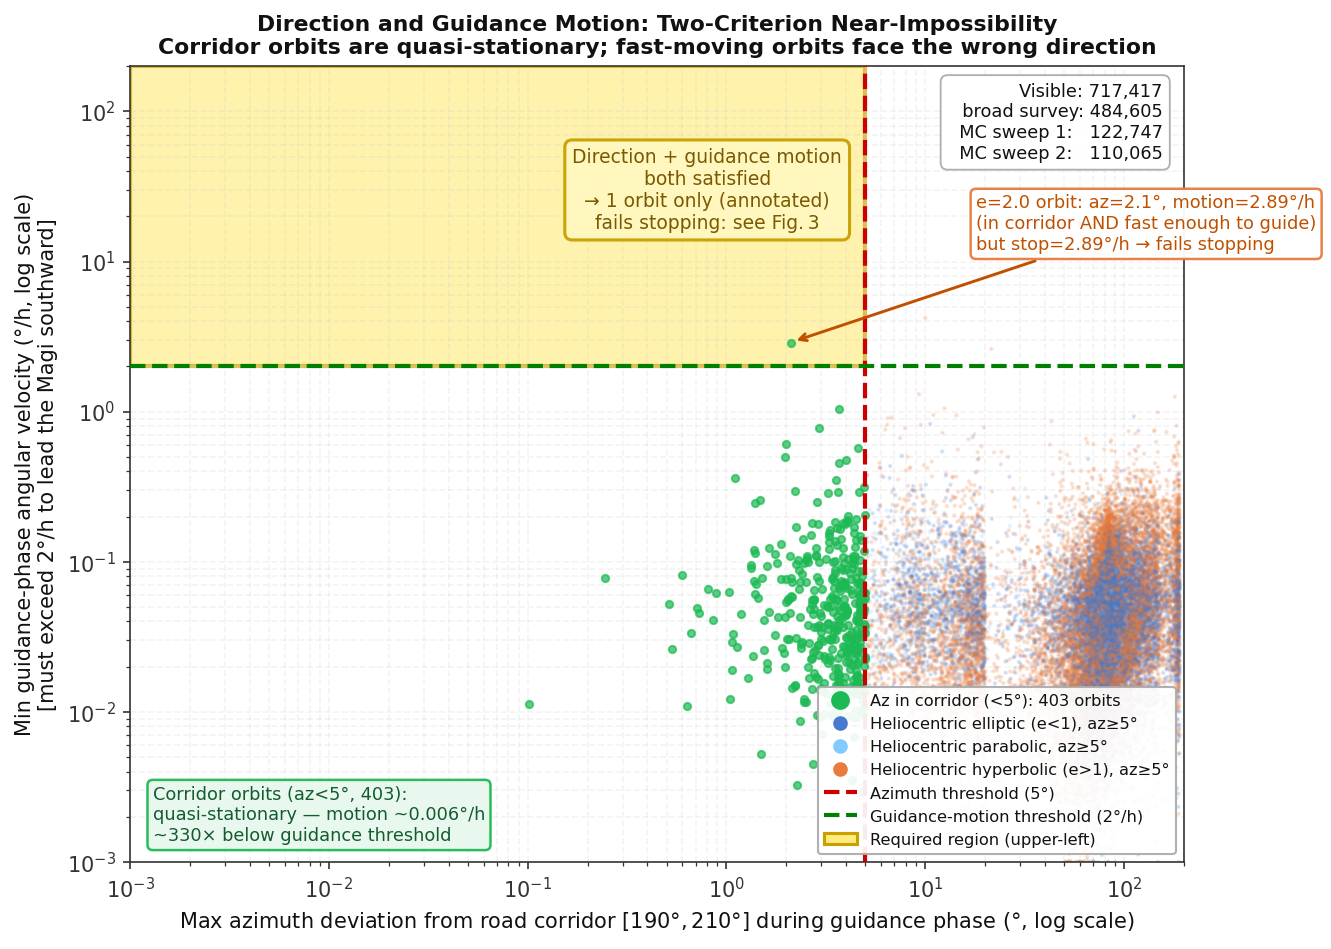
\includegraphics[width=\linewidth]{figure_paper2_az_motion}
  \caption{\textbf{Direction and guidance motion: two-criterion near-impossibility.}
    Each point is one visible orbital configuration from the full
    heliocentric parameter space (broad survey) and two Monte Carlo
    refinement sweeps. The horizontal axis (log scale) shows the maximum
    azimuth deviation of the object from the road corridor
    $[190^\circ,210^\circ]$ during the guidance phase (0 = perfectly in
    corridor); the vertical axis (log scale) shows the minimum angular
    velocity during that same phase (must exceed
    $2^\circ\,\mathrm{h}^{-1}$ to \grk{προάγειν}).
    A configuration satisfying both direction \emph{and} guidance motion
    simultaneously would fall in the gold-shaded upper-left region
    (azimuth deviation $<5^\circ$ \emph{and} motion
    $>2^\circ\,\mathrm{h}^{-1}$). That region is essentially empty:
    green points (corridor orbits, azimuth deviation $<5^\circ$) cluster
    along the bottom-left, quasi-stationary throughout with guidance
    speeds ${\sim}0.006^\circ\,\mathrm{h}^{-1}$ (factor ${\sim}330$
    below threshold); fast-moving orbits (upper right) are far outside
    the road corridor. The single annotated outlier ($e=2.0$,
    $\Delta\mathrm{az}=2.1^\circ$, motion $= 2.89^\circ\,\mathrm{h}^{-1}$)
    does enter the gold region but fails the third (stopping) criterion,
    as shown explicitly in Fig.~\ref{fig:scatter}.}
  \label{fig:azmotion}
\end{figure}

\begin{figure}[htbp]
  \centering
  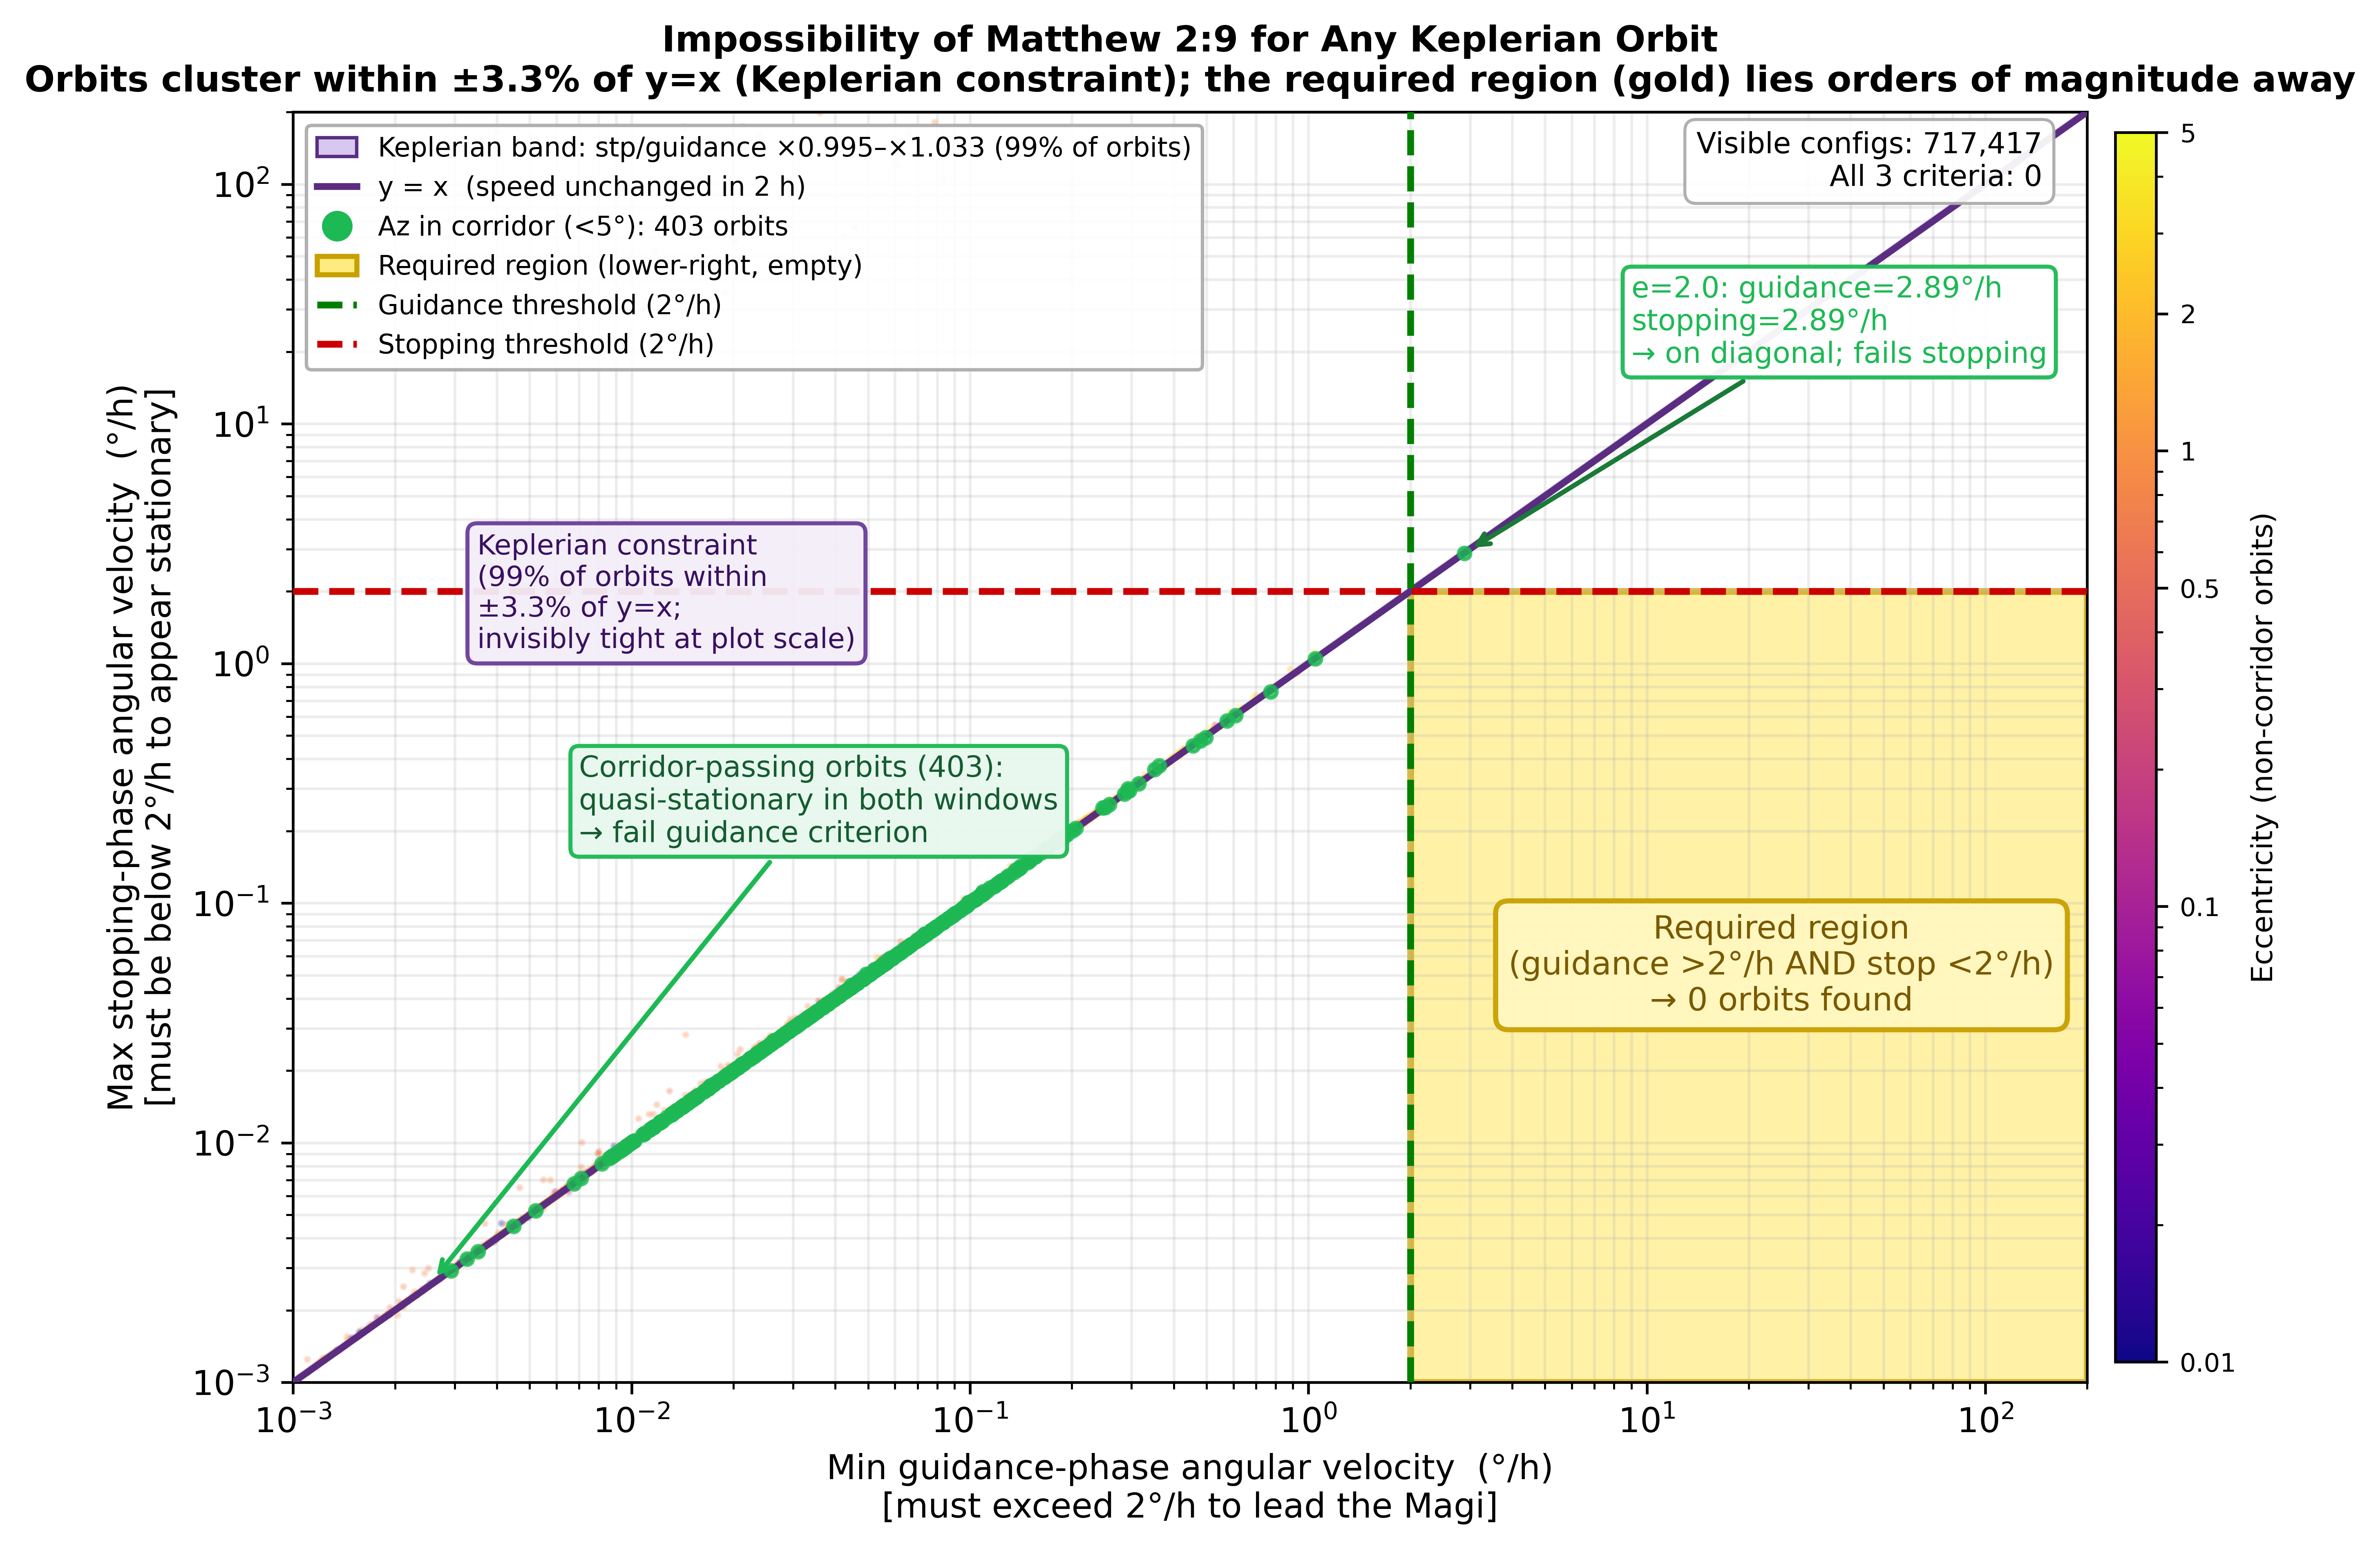
\includegraphics[width=\linewidth]{figure_paper2_impossibility_scatter_v2}
  \caption{\textbf{Orbital impossibility of Matthew 2:9.}
    Each point represents one visible orbital configuration sampled from the
    full heliocentric parameter space (broad survey) and two Monte Carlo
    refinement sweeps; non-corridor points are coloured by eccentricity
    (plasma scale). The horizontal axis (log scale) shows the
    \emph{minimum} angular velocity during the guidance phase
    (08:00–10:00 local time; must exceed $2^\circ\,\mathrm{h}^{-1}$ to
    lead the Magi southward). The vertical axis (log scale) shows the
    \emph{maximum} angular velocity during the subsequent stopping phase
    (10:15–12:00; must fall \emph{below} $2^\circ\,\mathrm{h}^{-1}$ to
    appear stationary over Bethlehem). A configuration satisfying
    \grk{προάγειν} and \grk{ἐστάθη} simultaneously would occupy the
    gold-shaded \emph{lower-right} region; that region contains zero orbits
    across every eccentricity class.
    The purple diagonal band is the \emph{Keplerian constraint}: the
    1st--99th percentile of the empirical stopping-to-guidance speed ratio,
    spanning only $\times 0.995$--$\times 1.033$ around $y=x$.
    Over any two-hour window the apparent angular velocity
    $\omega_\mathrm{app} = V_\perp/d$ changes by at most ${\lesssim}\,4\%$
    for heliocentric bodies (Supplementary \S\,S1.8); all points therefore
    cluster invisibly close to the diagonal.
    The required region lies orders of magnitude from this band, making the
    exclusion structural rather than a consequence of sparse sampling.
    Green points (azimuth deviation $<5^\circ$, in-corridor) cluster near
    the origin: quasi-stationary throughout both phases, confirming the
    anti-correlation visible in Fig.~\ref{fig:azmotion}. The single
    annotated outlier ($e=2.0$, $\Delta\mathrm{az}=2.1^\circ$) reaches
    $2.89^\circ\,\mathrm{h}^{-1}$ during guidance but retains the same
    speed during stopping, placing it on the diagonal and well above the
    stopping threshold.
    Supplementary Fig.~S1 shows each MC sweep separately.}
  \label{fig:scatter}
\end{figure}

%% tab:survey moved to Extended Data Table 1 (see end of manuscript)

\subsection{Orbit inversion confirms incompatibility}\label{subsec:inversion}

As a complementary test, I searched for the orbit that best fits the
guidance-phase sky positions, then propagated it into the stopping window.
Using a fine grid ($5^\circ$ spacing in $\Omega$ and $\omega$) over the
full eccentricity range ($e = 0$--$5.0$), the best-fitting guidance orbit
achieves an azimuth corridor score of $0.015^\circ$, within the corridor, yet fails
the guidance-motion criterion by an order of magnitude
($0.23^\circ\,\mathrm{h}^{-1}$ versus the required $2^\circ\,\mathrm{h}^{-1}$).
When this orbit is propagated into the stopping window, the object rapidly sets
below the horizon, the antithesis of the text's requirement
(Extended Data Fig.~1).

%% fig:proof moved to Extended Data Fig.~1 (see end of manuscript)

\subsection{Corpus-linguistic analysis: Matthew 2:9 vocabulary is
  incompatible with Greek astronomical and astrological discourse}
\label{subsec:linguistics}

The physical impossibility established above is independently corroborated by
a statistical analysis of ancient Greek astronomical vocabulary. If Matthew
2:9 described a real astronomical phenomenon, its language should conform to
the technical register shared by Greek astronomical and astrological texts.
I assembled a corpus of 24 texts (mathematical astronomy, astrological
application, and didactic popularizations) comprising approximately 619,000
words, spanning the fourth century~BCE through the fourth century~CE
(Supplementary Table~S7; Methods).

I identified four genre-register features of Matthew 2:9 that any
astronomical interpretation must implicitly assume, testing not merely lexical
choice but whether the narrative events they encode appear anywhere in
astronomical writing:
\begin{enumerate}
  \item[(A)] \grk{προάγω} (\tr{proag\={o}}): a star leading human
    travelers toward a destination.
  \item[(B)] \grk{ἵστημι} (\tr{hist\={e}mi}): a celestial body coming to
    rest \emph{above a terrestrial place}, as distinct from the zodiacal
    station the verb denotes in technical usage.
  \item[(C)] \grk{ἐπάνω} (\tr{epan\={o}}): rather than \grk{ὑπὲρ}:
    a celestial body localized above a specific terrestrial address.
  \item[(D)] \grk{ἔρχομαι} (\tr{erchomai}): a celestial body
    ``arriving'' at a specific location on Earth.
\end{enumerate}

All four Matthew-type usages score zero in the 619,000-word corpus
(Table~\ref{tab:linguistics}; passage-level citations in Supplementary
Table~S8). Feature~A: all 11 corpus occurrences of \grk{προάγω} carry
positional or temporal senses (``preceding in longitude''), never narrative
guidance ($p = 0.083$). Feature~B: all 121 occurrences of \grk{ἵστημι} place
a celestial body in a zodiacal sign, a degree, an aspect, a chart angle or
beside a fixed star, and never above a house, city or person ($p = 0.008$);
Matthew's own form \grk{ἐστάθη} does not occur in the corpus at all.
Feature~C: all 40 occurrences of \grk{ἐπάνω}
carry geometric or zodiacal senses, never localizing a body above a named
place ($p = 0.024$). Feature~D: \grk{ἔρχομαι} is used constantly of celestial
bodies arriving, 356 occurrences, but what they arrive at is always another
body or a point in the chart (``Mars \emph{coming upon} the Sun''; ``Jupiter
\emph{coming into} the horoskopos''), never a place on the ground
($p = 0.003$; a thematic robustness check yields the same result at every
feature, Supplementary Information, Table~S9). The joint Fisher combined
statistic is $\chi^2(8)=33.8$, $p \approx 4.5\times10^{-5}$
(Fig.~\ref{fig:linguistics}); Gaussian copula correction
($2\times10^6$ Monte Carlo draws) maintains significance across the whole
range of inter-feature correlation tested, to $\rho = 0.95$, and every
drop-one-feature subset remains jointly significant ($p < 0.05$).

\begin{table}[h]
\caption{Corpus linguistics: Fisher's exact test of Matthew 2:9 vocabulary
  against Greek astronomical and astrological texts.}\label{tab:linguistics}
\begin{tabular}{@{}llccc@{}}
\toprule
Feature & Matthew usage & Corpus count & Matthew & $p$ (Fisher) \\
\midrule
(A) \grk{προάγω}             & Guidance of travelers       & 0\,/\,11   & 1  & $0.083$ \\
(B) \grk{ἵστημι}             & Celestial body halts above a place & 0\,/\,121  & 1  & $0.008$ \\
(C) \grk{ἐπάνω}              & Above specific earthly point & 0\,/\,40   & 1  & $0.024$ \\
(D) \grk{ἔρχομαι}            & Spatial arrival of Star      & 0\,/\,356  & 1  & $0.003$ \\
\midrule
\textbf{Joint (A–D)} & --- & --- & --- & \begin{tabular}[t]{@{}l@{}} $\mathbf{\chi^2(8)=33.8,}$ \\ $\mathbf{p \approx 4.5\times10^{-5}}$ \end{tabular} \\
\bottomrule
\end{tabular}
\footnotetext{Corpus: 24 texts, $\approx\!619{,}000$ words, 4th~c.~BCE–4th~c.~CE
(see Supplementary Table~S7). TLG counts, 2026-09-04 (MIT IRIS proxy),
by exact wordform search over the full paradigm of each lemma, with
\textsf{Exact Match} and \textsf{Diacritics sensitive} enabled;
see Supplementary Table~S8 for passage-level citations.
Fisher's exact test, one-sided: $p = 1/(N+1)$, where $N$ = corpus negatives.
``Corpus count'' shows Matthew-type positive\,/\,non-Matthew-type negative hits.
All four Matthew-type usages score zero in the corpus.
\grk{Ἔρχομαι} is suppletive; all four stems
(\grk{ἐρχ-}, \grk{ἐλευσ-}, \grk{ἐλθ-/ἠλθ-}, \grk{ἐληλυθ-}) were searched,
including the aorist that supplies Matthew's own \grk{ἐλθών}.
Joint row reports Fisher's combined
$\chi^2 = -2\sum\ln p_i = 33.8$ with $\mathrm{df}=8$, $p\approx4.5\times10^{-5}$;
corrected for inter-feature
correlation by Gaussian copula: $\rho = 0.5$ yields $p = 0.0027$; significance
maintained across the whole tested range, to $\rho = 0.95$
(Supplementary Information, Section~3).}
\end{table}

The null result is uniform across genre: even astrological texts (Ptolemy's
\textit{Tetrabiblos}, Vettius Valens, Hephaestion), the most likely to adopt
narrative vocabulary, use \grk{φέρεσθαι}/\grk{κινεῖσθαι} and \grk{ὑπὲρ}
throughout; Matthew's guidance vocabulary is absent from mathematical and
astrological texts alike (Supplementary Information).
This result is independently corroborated by Schironi's philological survey of
ancient Greek astronomical terminology\cite{schironi2024}, which identifies as
the standard technical vocabulary for celestial leading/preceding:
\grk{ἡγούμενος}/\grk{προηγούμενος} (not \grk{προάγω}); and for a body located
above a zodiacal band: \grk{ὑπέρ} (not \grk{ἐπάνω}). For stationary points
Schironi gives \grk{στηρίζω}/\grk{στηριγμοί}, and the corpus shows
\grk{ἵστημι} serving the same technical sense: Geminus glosses planets
``standing still'' as what ``they call \grk{στηριγμούς}''. The distinction
that bears on Matthew~2:9 is accordingly not which verb is chosen but what it
governs, and in the corpus that is never a terrestrial place.
The documentary horoscopes and astronomical papyri from Oxyrhynchus\cite{jones1999}
confirm the same conventions in applied astrological practice, extending the
vocabulary evidence beyond literary texts to working astronomical documents.

\begin{figure}[htbp]
  \centering
  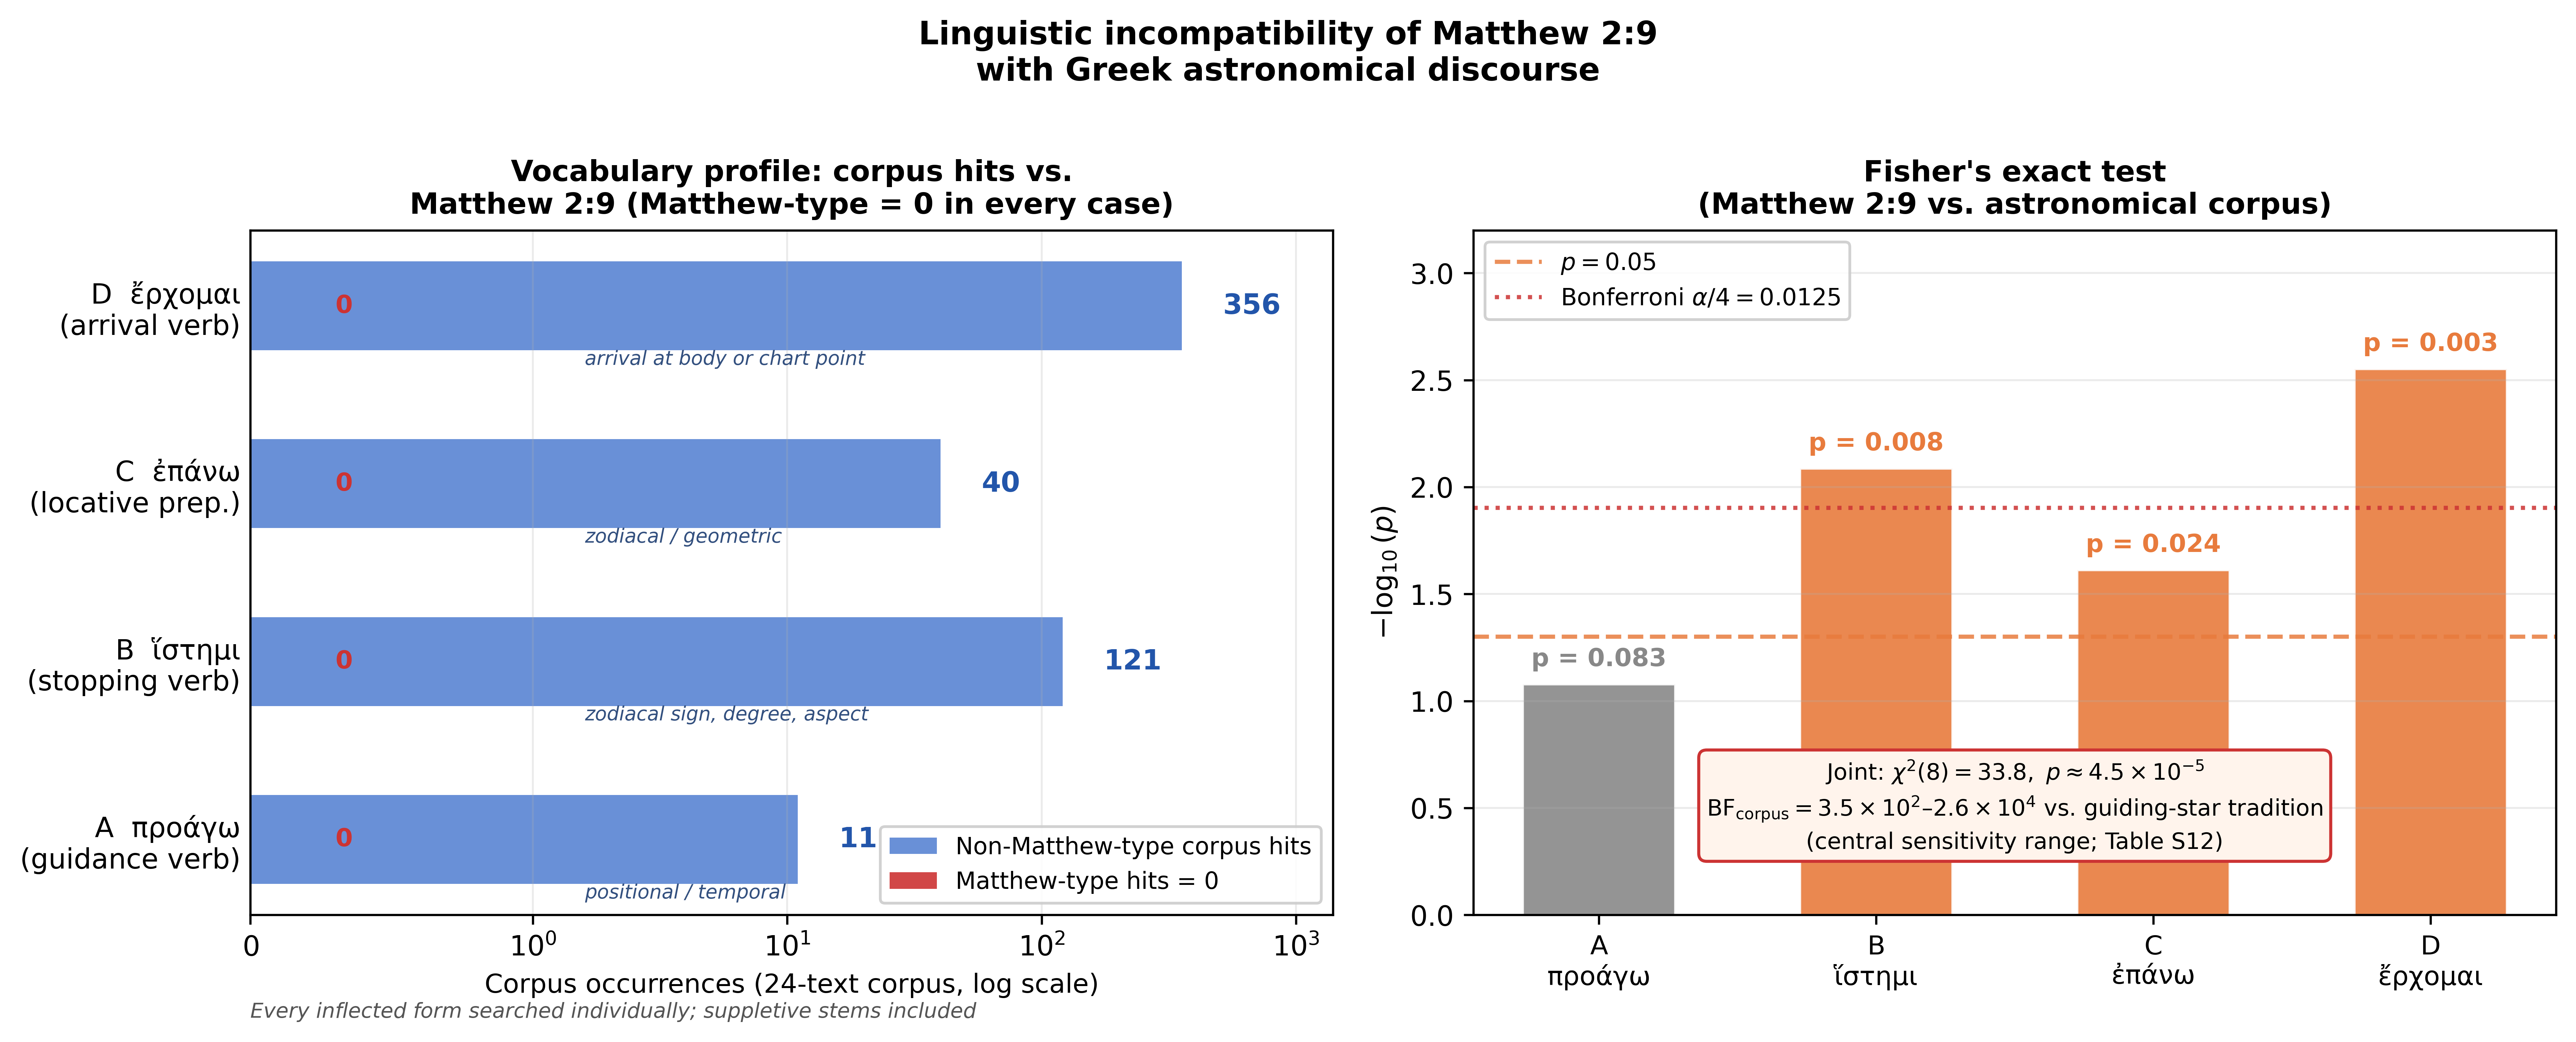
\includegraphics[width=\linewidth]{figure9_corpus_linguistics}
  \caption{\textbf{Linguistic incompatibility of Matthew 2:9 with Greek
    astronomical discourse.} TLG counts, 2026-09-04, by exact wordform
    search over the full paradigm of each lemma.
    \textbf{Left},~Corpus hit counts for each lemma (blue bars, 11--356
    occurrences); the Matthew-type usage (red square) scores zero in
    every case: no hit in the 24-text corpus ($\approx\!619{,}000$ words)
    belongs to the narrative sense Matthew employs.
    \textbf{Right},~Fisher's exact test: $-\log_{10}(p)$ for each of the
    four features; dashed orange line marks $p = 0.05$, dotted red line
    the Bonferroni threshold ($\alpha/4 = 0.0125$). Features~B
    (\grk{ἵστημι}), C (\grk{ἐπάνω}) and~D (\grk{ἔρχομαι}) individually cross
    $p = 0.05$, and B and D also cross the Bonferroni threshold; the joint Fisher
    combined statistic is $\chi^2(8) = 33.8$, $p \approx 4.5\times10^{-5}$,
    and every drop-one subset remains jointly significant.
    The corpus includes both mathematical astronomy and astrological texts;
    the absence of Matthew's vocabulary is uniform across all genres.}
  \label{fig:linguistics}
\end{figure}

\subsection{Bayes factor: Matthew 2:9 vocabulary matches the guiding-star
  narrative tradition}\label{subsec:bayes}

The corpus analysis above establishes that Matthew's four-feature vocabulary
is improbable under the astronomical hypothesis (Fisher combined $p \approx 4.5\times10^{-5}$).
A complementary question is whether that vocabulary is probable under the
alternative hypothesis that Matthew~2:9 belongs to the ancient guiding-star
narrative tradition~(\textit{H}\textsubscript{guide}). Four independent traditions
attest this genre: Virgil's \textit{Aeneid}~2.687--711 (Servius \textit{ad
Aen.}~2.694 identifies the guide as Venus/Lucifer, the morning star); Plutarch
and Diodorus Siculus on the Timoleon guiding light; Lucian's
\textit{Navigium}~7,~9 (explicitly a star); and the LXX pillar-of-fire
(\textit{Exodus}~13.21; \textit{Wisdom}~10.17 describes it as star-like at night) 
\cite{adair2012,adair_jsnt,heilen2015}. Each involves a divinely-sent luminous guide.
I scored each tradition for features A--D and estimated
$P(\text{feature}_i \mid H_\text{guide})$ with Laplace smoothing
($k=1$, $N=4$; Supplementary Table~S11).
Feature~A is present in all four traditions; D in three; B in two;
C in two (Lucian's \grk{ἐπικαθίσαι τῷ καρχησίῳ} and the Israelite pillar standing \grk{ἐπί} 
the Tabernacle, both using the same \grk{ἐπι-} root as Matthew's \grk{ἐπάνω}).
Under the independence approximation:
\begin{equation}
  P(A,B,C,D \mid H_\text{guide}) = \prod_{i} P_i \approx 1.39\times10^{-1}.
  \label{eq:pguide}
\end{equation}
The Bayes factor comparing the guiding-star hypothesis to the astronomical
hypothesis is therefore:
\begin{equation}
  \mathrm{BF} = \frac{P(A,B,C,D \mid H_\text{guide})}
                      {P(A,B,C,D \mid H_\text{astro})}
             = \frac{1.39\times10^{-1}}{4.67\times10^{-8}}
             \approx 3.0\times10^{6}.
  \label{eq:bf}
\end{equation}
Here $P(A,B,C,D\mid H_\text{astro}) = \prod_i p_i = 4.67\times10^{-8}$ is
the product of the four individual Fisher exact probabilities, the correct
joint data probability under independence, rather than the Fisher combined
meta-test tail probability ($4.5\times10^{-5}$), which is a test statistic,
not a joint data probability.
This BF exceeds 100 on the Jeffreys scale, providing strong evidence in favor of
the guiding-star narrative hypothesis over the astronomical one. Sensitivity analyses confirm robustness. Varying the corpus composition by
adding four additional omen texts gives $\mathrm{BF} = 5.1\times10^{5}$; varying the
Laplace smoothing parameter $k \in [0.5, 3]$ gives
$\mathrm{BF} \in 2.3$--$3.4\times10^{6}$; a 3$\times$ denominator uncertainty
yields a range of $1.0$--$9.3\times10^{6}$
(Supplementary Table~S11).

Feature~C (\grk{ἐπάνω}) is particularly diagnostic: every astronomical and
omen text examined uses \grk{ὑπὲρ} for a celestial body above a terrestrial
point, including Josephus (\textit{JW}~6.289) and Dio Cassius (54.29.8),
both of whom use \grk{ἵστημι}/\grk{αἰωρέω} with \grk{ὑπὲρ};
\grk{ἐπι}-based localization is attested in the present corpus only in
legendary and sacred narrative texts (Lucian; \textit{Joseph and Aseneth}~14.4;
the Israelite pillar-of-fire tradition, where \grk{ἐπί} marks the cloud
standing over the Tabernacle: Exod~40.38, Num~9.15, 9.18--22). This
distributional split confirms the Bayes factor at the individual-feature level
(Supplementary Information).

%%%% =======================================================================
\section{Discussion}\label{sec:discussion}
%%%% =======================================================================

The foregoing analysis produces three convergent results.
\textit{First}, Matthew's own vocabulary establishes an internal prima facie
case: across 118 other Matthean occurrences of the four motion words, zero
appear in an astronomical sense, yielding $\mathrm{BF}_\text{Matthew} \approx
88{,}000$ against the astronomical reading from the author's idiolect alone.
\textit{Second}, orbital mechanics closes the ``loose-language'' escape route:
no Keplerian body can exhibit both the sustained guidance motion and the
punctual stopping, confirmed by a kinematic argument, a survey of
529~million heliocentric and 28,800 geocentric configurations finding zero
solutions, Monte Carlo refinement, and a targeted close-flyby search.
\textit{Third}, external corpus-linguistic analysis delivers the positive
genre classification: Matthew's four-feature vocabulary is unattested in
the surveyed ${\approx}\,619{,}000$-word astronomical corpus while fitting the
narrative tradition at $\mathrm{BF}_\text{corpus} \approx 3.0\times10^{6}$
under strict independence. Because the internal and external linguistic
datasets are entirely disjoint, their Bayes factors are treated as
conditionally independent of one another; both are nonetheless products over
the same four features of a single clause, so the joint factor is reported as
a sensitivity range. At the independence corner of Supplementary
Table~\ref{tab:bfsens} it is $87{,}696 \times 3.0\times10^{6} \approx
2.6\times10^{11}$; at the opposite corner, with within-feature clustering and
between-feature dependence both at their strongest, it is
${\approx}\,6.4\times10^{3}$. Every cell of the grid remains decisive, and
the range is reported in full rather than collapsed to a single figure.
This linguistic classification is independent of the orbital mechanics.

Previous studies operated within a \emph{search} paradigm, identifying the
best-matching historical event. The present work operates within a
\emph{demonstration} paradigm: deriving kinematic requirements and showing that the
feasible set is empty. A failed search leaves open the possibility of an
undiscovered candidate; an empty feasible set eliminates the entire class
simultaneously. The conclusion is robust to reference date (verified across all
major proposed epochs, 12~BCE to 1~BCE), journey duration (1--4~h), and
azimuthal tolerance (null result holds at $15^\circ$), extending across every
orbit type: elliptic, parabolic, hyperbolic, heliocentric, and geocentric.

A recent systematic review of proposals concluded that all purely
astronomical candidates were effectively eliminated; this left a different sort of approach based
on the Jupiter horoscope of 17~April 6~BCE (Molnar's astrological reading) as the ``leading and default
explanation''\cite{schaefer2015,schaefer2015molnar}. The present analysis, however,
extends the impossibility beyond astronomical candidates to close any remaining
opening in that position, demonstrating that the fault is not in the stars but in the astrological theories themselves.
First, the kinematic demonstration applies equally to Jupiter during its
6~BCE apparition: the planet's apparent angular velocity (${\approx}\,0.035^\circ\,\mathrm{h}^{-1}$
relative to background stars, far below the $2^\circ\,\mathrm{h}^{-1}$ threshold)
satisfies the stopping criterion throughout its entire synodic period: it
cannot \grk{προάγειν} (``go before'') anything, let alone travelers, in any kinematically
meaningful sense on the timescale the narrative implies. The same can be said for any other planet. 
Second, the astrological reading of Matt~2:9 depends on a ``loose language''
escape: it requires the Greek verbs to describe not the Star's apparent sky
motion but an astrological configuration.
The corpus-linguistic analysis closes this exit: \grk{προάγω}, \grk{ἵστημι},
\grk{ἐπάνω}, and \grk{ἔρχομαι} are absent from the astrological sub-corpus
(Ptolemy \textit{Tetrabiblos}, Vettius Valens, Hephaestion, Dorotheus,
Pseudo-Manetho, Paul of Alexandria) in exactly the Matthew-type senses,
confirming that the vocabulary belongs to the narrative guiding-star register
rather than the astrological one. All of Molnar's deductions about the Greek of Matt~2:9, 
which Schaefer depends on, are without philological foundation\cite{birdsall2002,heilen2015,adair2013star}. 
Third, Schaefer characterizes the skeptical position, that Matthew~2:9 is legendary, as
having ``no evidence in its favor, and having explained none of the details or
coincidences''\cite{schaefer2015molnar}.
This characterization overlooks a substantial body of New Testament scholarship: the majority critical position, 
represented by Brown\cite{brown1993} and reinforced in the same Brill volume by Merz, who co-authored the standard 
historical-Jesus reference work\cite{merz2015}, holds that the infancy narratives are literary constructions rather than historical reports.
The present paper provides that evidence quantitatively: a Bayes factor that is
decisive on the Jeffreys scale under every dependence assumption tested,
indicating a non-physical and a specifically legendary motif,
and a kinematic demonstration that no physically real object can satisfy the text's requirements at any epoch.

Non-gravitational forces cannot rescue the astronomical interpretation.
`Oumuamua's anomalous acceleration (${\approx}\,5\times10^{-9}$\,km\,s$^{-2}$;
\cite{micheli2018}), the largest known, delivers at most
$\Delta v \approx 3.6\times10^{-5}$\,km\,s$^{-1}$ over 2\,h, a factor of
${\approx}\,4\times10^4$ below the 1.5\,km\,s$^{-1}$ required at closest
approach ($d\approx0.003$\,AU), and ${\approx}\,3\times10^7$ below the
requirement at $d \gtrsim 0.1$\,AU. No chemically plausible force bridges
this gap in any orbital regime.

A common retreat reads the verbs loosely: \grk{προῆγεν} as static
``ahead of'' and \grk{ἐστάθη} as conveniently placed at journey's end.
This is grammatically impermissible\cite{adair2013star}, and the corpus
results undermine it regardless: the analysis tests whether the vocabulary
belongs to the astronomical register, and it does not: \grk{προάγω},
\grk{ἔρχομαι}, \grk{ἵστημι} with a terrestrial complement, and
\grk{ἐπάνω} (rather than \grk{ὑπὲρ}) are all anomalous in astronomical
writing. A looser reading reinforces, not dissolves, the linguistic evidence.

The three lines of evidence are mutually reinforcing: the mechanics shows the
motion is physically impossible; the internal linguistics shows Matthew never
uses these words astronomically; the external linguistics shows the vocabulary
belongs to a different register. Thematically, active stellar guidance to a
specific address and stopping above it is unattested in the texts examined,
while it recurs in the guiding-star legend tradition (Supplementary
Information). Feature~C (\grk{ἐπάνω}) is particularly diagnostic: every
astronomical and omen text in the present corpus employs \grk{ὑπὲρ} for a
celestial body above a terrestrial point; \grk{ἐπι}-localization is attested
in the present corpus only in legendary narrative texts (Supplementary
Information).

The result bears exclusively on Matthew~2:9. The companion verse Matthew~2:2
imposes additional constraints (a potential heliacal rising requires solar
proximity) not analyzed here; my analysis is
deliberately conservative in ignoring them. The conclusion rests on the
assumption shared by every naturalistic proposal in the literature: that the
narrative intends a physically real object whose motion can be described in
astronomical terms. Within that assumption, the present analysis finds no
viable astronomical candidate across any eccentricity class or orbit type.

\textbf{Scope and limitations.}
Four boundaries deserve emphasis. First, the impossibility applies to the
literal astronomical reading of Matthew~2:9; allegorical or symbolic
literary readings are not constrained. Second, non-Keplerian physics is
considered but not exhaustively modeled: the primary impossibility (transverse
velocities $\sim\!10^3$--$10^4$\,km\,s$^{-1}$) is insensitive to any
chemically plausible non-gravitational force, but arbitrarily exotic objects
are not formally excluded. Third, Matthew~2:2 is excluded from the orbital
survey; that verse may independently constrain candidate objects or further indicate 
other culturally relevant details. Fourth, nothing can be determined 
about the origins of the narrative, if it was inherited by the Gospel author or was their 
own invention, from this analysis. Independent studies are needed to address source-critical 
questions, including the adoption of a prior ``morning star'' tradition concerning Jesus\cite{adair_jsnt}.

\textbf{Broader applicability.}
The demonstration framework introduced here is generalizable beyond Matthew~2:9.
The companion verse Matthew~2:2 independently constrains any candidate to
solar-proximity orbits (a heliacal rising requires the object to have been near
the sun in preceding weeks), a restriction deliberately excluded from the
present survey whose addition would only strengthen the null result.
More broadly, any ancient text whose astronomical interpretation requires
specific celestial kinematics can in principle be subjected to the same
two-step analysis: an exhaustive orbital parameter-space survey establishing
what is kinematically possible, followed by a corpus-register test establishing
whether the vocabulary belongs to the astronomical genre.
Ancient omen literature, East Asian annals used to date historical comets,
and other sky-event narratives for which both physical constraints and
comparative textual corpora exist are natural applications of this combined framework.

%%%% =======================================================================
%% REQUIRED NATURE SECTIONS
%%%% =======================================================================

\section*{Data availability}
The Greek corpus search results, TLG hit records, and Monte Carlo output data
supporting this study are available in the GitHub repository at
\url{https://github.com/adairaar/sob_astro_test}.

\section*{Code availability}
All Python scripts used for the orbital-mechanics surveys, Monte Carlo
analyses, and corpus-linguistic calculations are available at
\url{https://github.com/adairaar/sob_astro_test}. Full reproduction
instructions are provided in the repository \texttt{README}.

\section*{Author contributions}
A.A.\ conceived the study, designed and implemented all orbital-mechanics and
corpus-linguistic analyses, produced all figures and tables, and wrote the
manuscript.

\section*{Competing interests}
The author declares no competing interests.

\section*{Acknowledgements}
This research received no external funding.

%%%% =======================================================================
%% BIBLIOGRAPHY
%%%% =======================================================================

\bibliography{sob_refs}

%%%% =======================================================================
%% EXTENDED DATA
%% Nature allows up to 10 Extended Data figures/tables (not counted in the
%% 6 display-item limit for the main text).
%%%% =======================================================================

\clearpage
\setcounter{table}{0}
\renewcommand{\thetable}{\textbf{Extended Data Table~\arabic{table}}}
\setcounter{figure}{0}
\renewcommand{\thefigure}{\textbf{Extended Data Fig.~\arabic{figure}}}

%%-----------------------------------------------------------------------, 
%% Extended Data Table 1  (was tab:survey in main text)
%%, -----------------------------------------------------------------------
\begin{table}[h]
\caption{\textbf{Orbital survey results: configurations sampled, azimuth
  corridor pass counts, and best guidance angular velocity, by orbit class
  (primary epoch JD~1\,719\,755.9, 5~BCE).}
  ``Azimuth pass'' = number of visible configurations whose azimuth
  remains within the road corridor $[190^\circ,\!210^\circ]\pm5^\circ$
  throughout the entire 2\,h guidance window.
  ``Best $\omega_\text{guide}$'' = maximum guidance-phase angular velocity
  among all azimuth-passing configurations.
  No configuration satisfies the azimuth, guidance-motion, \emph{and}
  stopping criteria simultaneously.
  Full parameter grids are given in Supplementary Table~S2.}
\label{tab:survey}
\begin{tabular}{@{}lrrrr@{}}
\toprule
Orbit class & Configs sampled & Azimuth pass & Best $\omega_\text{guide}$
  ($^\circ$\,h$^{-1}$) & All criteria \\
\midrule
Heliocentric (all types) & 529,079,040 & 126,720 & $\leq 0.04$ & 0 \\
\quad Elliptic ($e<1$)   & 352,719,360 & $\approx\!84{,}500$ & $\leq 0.04$ & 0 \\
\quad Parabolic ($e=1$)  & 35,271,936  & $\approx\!8{,}400$  & $\leq 0.04$ & 0 \\
\quad Hyperbolic ($e>1$) & 141,087,744 & $\approx\!33{,}800$ & $\leq 0.04$ & 0 \\
Geocentric (LEO–lunar)   & 28,800      & \multicolumn{1}{c}{---$^\dagger$}
  & \multicolumn{1}{c}{---} & 0 \\
\midrule
\textbf{Total visible}   & \textbf{202,400,876} & \textbf{126,720} &
  $\leq\mathbf{0.04}$ & \textbf{0} \\
\bottomrule
\end{tabular}
\footnotetext{Census columns (configurations sampled, azimuth pass) carry a
tolerance of ${\approx}0.1\%$ and ${\approx}0.3\%$ respectively, reflecting
configurations that lie within numerical noise of a threshold and may be
classed either way under different ephemeris implementations
(Supplementary~\S\,\ref{subsec:reproducibility}).  The final column is exact: it is zero under every
build tested.
Guidance window: 08:00--10:00 local time (9 steps at
15\,min spacing); stopping window: 10:15--12:00 (8 steps).
Azimuth corridor: $[190^\circ, 210^\circ]$, road bearing Jerusalem to
Bethlehem; pass criterion: maximum azimuth deviation $<\!5^\circ$ from
corridor boundary throughout entire guidance window.
Guidance-motion criterion: minimum apparent angular velocity
$> 2^\circ\,\mathrm{h}^{-1}$; stopping criterion:
maximum apparent angular velocity $< 2^\circ\,\mathrm{h}^{-1}$.
Visibility: altitude $> 5^\circ$ (analysis covers daylight hours; no twilight constraint applied).
Sub-class visible and azimuth-pass counts are proportional estimates
(10:1:4 ratio of $e$-values sampled; the total row gives verified counts).
Monte Carlo refinement ($2.25\times10^6$ draws around the best-fit grid
orbit) confirmed zero solutions; best guidance motion among
azimuth-passing configurations in any sweep $\leq 0.006^\circ\,\mathrm{h}^{-1}$,
a factor of ${\sim}330$ below the $2^\circ\,\mathrm{h}^{-1}$ threshold.
The $0.23^\circ\,\mathrm{h}^{-1}$ figure cited in the text is from the
separate fine-grid orbit inversion (Section~\ref{subsec:inversion}), which
minimises integrated azimuth deviation; that orbit temporarily exits the
corridor at some time steps within the window, so it is not counted as an
azimuth pass here.
The annotated outlier ($e=2.0$, Fig.~\ref{fig:azmotion}) satisfies the
corridor and guidance-motion criteria instantaneously but does not sustain
corridor confinement throughout the full 2\,h window, so it likewise does not
appear in the azimuth-pass count.\\
$^\dagger$\,Geocentric survey used ground-frame (AltAz) angular velocity.
The Moon (only natural geocentric body) peaks at $\omega = 0.61^\circ\,\mathrm{h}^{-1}$
at perigee, below the $2^\circ\,\mathrm{h}^{-1}$ guidance threshold.
A comprehensive survey of 28,800 hypothetical geocentric configurations finds
zero satisfying all criteria with $\omega_\mathrm{stop} < 0.20^\circ\,\mathrm{h}^{-1}$;
see Supplementary~\S\,S1.10.}
\end{table}

%%-----------------------------------------------------------------------, 
%% Extended Data Fig. 1  (was fig:proof in main text)
%%, -----------------------------------------------------------------------
\begin{figure}[htbp]
  \centering
  \includegraphics[width=\linewidth]{figure6_impossibility_proof}
  \caption{\textbf{Orbit inversion demonstration that guidance and stopping
    are mutually exclusive.}
    a)~Best heliocentric orbit that maximizes southward
    apparent motion during the guidance phase (red arc). At the
    guidance epoch the object is above the horizon (altitude $>10^\circ$)
    and moving southward at $> 2^\circ\,\mathrm{h}^{-1}$.
    b)~The same orbit propagated forward to the stopping epoch.
    The object has set below the horizon ($< 0^\circ$ altitude; shown as
    dashed trajectory), violating the visibility requirement.
    No orbit simultaneously satisfies guidance motion, stopping, azimuth,
    and visibility at both epochs. Orbit propagated via Barker's equation
    (parabolic) and Newton--Raphson Kepler-equation iteration (elliptic /
    hyperbolic); Earth position from JPL DE430; local horizontal frame
    at Bethlehem ($31.70^\circ$\,N, $35.20^\circ$\,E, 765~m).}
  \label{fig:proof}
\end{figure}

\end{document}
